\documentclass{beamer} \useoutertheme{infolines}
\usefonttheme{default}

\usepackage{xcolor}     % for defining colors
\usepackage{multicol}   % for multiple columns
\usepackage{etoolbox}   % for toggles
\usepackage{subcaption} % for subplots
\usepackage{listings}   % for colored verbatim
\usepackage{ifthen}     % for conditionals
\usepackage{booktabs}   % for different table rules (lines)
\usepackage{tikz}       % for tikz pictures
\usetikzlibrary{calc}   % for computing points in tikz pictures
% required packages
\usepackage{xcolor}
\usepackage{stmaryrd} % jump brackets: \llbracket, \rrbracket

% create a provideenvironment command
\makeatletter
\def\provideenvironment{\@star@or@long\provide@environment}
\def\provide@environment#1{%
  \@ifundefined{#1}%
    {\def\reserved@a{\newenvironment{#1}}}%
    {\def\reserved@a{\renewenvironment{dummy@environ}}}%
  \reserved@a
}
\def\dummy@environ{}
\makeatother

% general
\newcommand{\x}{\mathbf{x}}
\newcommand{\qpoint}{\x_q}
\newcommand{\timevalue}{t}
\newcommand{\timestepsize}{\Delta\timevalue}
\newcommand{\dt}{\timestepsize}
\newcommand{\timeindex}{n}
\newcommand{\speed}{v}
\newcommand{\velocity}{\mathbf{\speed}}
\newcommand{\velocityx}{u}
\newcommand{\normalvectorletter}{n}
\newcommand{\normalvector}{\mathbf{\normalvectorletter}}
\newcommand{\normalx}{\normalvectorletter_x}
\newcommand{\normaly}{\normalvectorletter_y}
\newcommand{\ndimensions}{N_\text{dim}}
\newcommand{\ncomponents}{N_\text{comp}}
\newcommand{\ndofs}{N_\text{dof}}
\newcommand{\nnodes}{N_\text{node}}
\newcommand{\dofindex}{j}
\newcommand{\nodeindex}{k}
\newcommand{\componentindex}{m}
\newcommand{\transpose}{^{\text{T}}}

% schemes
\newcommand{\low}{L}
\newcommand{\high}{H}

% solution
\newcommand{\scalarsolution}{u}
\newcommand{\vectorsolution}{\mathbf{\scalarsolution}}
\newcommand{\approximate}[1]{\tilde{#1}}
\newcommand{\approximatescalarsolution}{\approximate{\scalarsolution}}
\newcommand{\approximatevectorsolution}{\approximate{\vectorsolution}}
\newcommand{\solutionletter}{U}
\newcommand{\solutionvector}{\mathbf{\solutionletter}}
\newcommand{\U}{\solutionvector}
\newcommand{\lowordersolution}[1][]{
  \ifthenelse{\equal{#1}{}}{\solutionvector^L}{\solutionvector^{L,#1}}}
\newcommand{\highordersolution}[1][]{
  \ifthenelse{\equal{#1}{}}{\solutionvector^H}{\solutionvector^{H,#1}}}

% sets
\newcommand{\faces}{\mathcal{F}}
\newcommand{\quadraturepoints}{\mathcal{Q}}

% domain and FEM
\newcommand{\domain}{\mathcal{D}}
\newcommand{\celldomain}[1][\cell]{\domain_#1}
\newcommand{\facedomain}{\domain}
\newcommand{\domainboundary}{\partial\domain}
\newcommand{\incomingdomainboundary}{\domainboundary^{\text{inc}}}
\newcommand{\cellindex}{K}
\newcommand{\cell}{K}
\newcommand{\celldiameter}{\Delta x}
\newcommand{\maxcelldiameter}{\Delta x_{\text{max}}}
\newcommand{\volume}{V}
\newcommand{\dvolume}{\,d\volume}
\newcommand{\area}{A}
\newcommand{\darea}{\,d\area}
\newcommand{\testfunction}{\varphi}
\newcommand{\vectortestfunctionscalar}{\Phi}
\newcommand{\vectortestfunction}{\mathbf{\vectortestfunctionscalar}}
\newcommand{\support}{S}
\newcommand{\maxdof}{N}
\newcommand{\interpolant}{\Pi}

% local viscous bilinear form
\newcommand{\localvisc}{b}
\newcommand{\localviscbilinearform}[3]{\localvisc_#1(\testfunction_#2, \testfunction_#3)}
\newcommand{\cellvolume}{|\celldomain|}
\newcommand{\cardinality}[1][]{\ifthenelse{\equal{#1}{}}{n_\cell}{n_#1}}
\newcommand{\cardsystem}{\bar{n}}
\newcommand{\indices}{\mathcal{I}}
\newcommand{\indicesnode}{\indices^{\text{node}}_\cell}
\newcommand{\indicescell}[1][]{\ifthenelse{\equal{#1}{}}{\indices_{\cell}}
  {\indices_{#1}}}

% entropy viscosity
\newcommand{\entropy}{\eta}
\newcommand{\entropyflux}{\mathbf{\consfluxletter}^\eta}
\newcommand{\entropyjump}{\mathcal{J}}
\newcommand{\entropyresidual}{\mathcal{R}}
\newcommand{\entropyresidualcoef}{c_\entropyresidual}
\newcommand{\entropyjumpcoef}{c_\entropyjump}
\newcommand{\entropynormalization}{\hat{\entropy}}

% conservation law
\newcommand{\consfluxletter}{f}
\newcommand{\consflux}{\mathbf{\consfluxletter}}
\newcommand{\consfluxsystem}{\mathbf{\MakeUppercase{\consfluxletter}}}
\newcommand{\consfluxscalar}[1][\scalarsolution]{\mathbf{\consfluxletter}(#1)}
\newcommand{\consfluxvector}{\mathbf{\MakeUppercase{\consfluxletter}}}
\newcommand{\consfluxinterpolant}{\mathrm{F}}
\newcommand{\conssource}{\mathbf{s}}

% viscosity
\newcommand{\viscosity}{\nu}
\newcommand{\cellviscosity}{\viscosity_\cellindex}
\newcommand{\lowordercellviscosity}[1][]{
  \ifthenelse{\equal{#1}{}}{\cellviscosity^L}
  {\cellviscosity^{L,#1}}}
\newcommand{\highordercellviscosity}[1][]{
  \ifthenelse{\equal{#1}{}}{\cellviscosity^H}
  {\cellviscosity^{H,#1}}}
\newcommand{\entropycellviscosity}[1][]{
  \ifthenelse{\equal{#1}{}}{\cellviscosity^\entropy}
  {\cellviscosity^{\entropy,#1}}}

% viscous fluxes
\newcommand{\viscstring}{\text{visc}}
\newcommand{\viscflux}[1]{\mathbf{\consfluxletter}^{\viscstring,#1}}
\newcommand{\viscconsfluxvector}
  {\mathbf{\MakeUppercase{\consfluxletter}}^\viscstring
  (\vectorsolution,\viscosity)}

% mass matrix
\newcommand{\massmatrixletter}{M}
\newcommand{\massmatrix}{\mathbf{\massmatrixletter}}
\newcommand{\M}{\massmatrix}
\newcommand{\consistentmassmatrix}{\massmatrix^C}
\newcommand{\consistentmassentry}{\massmatrixletter^C_{i,j}}
\newcommand{\lumpedmassmatrix}{\massmatrix^L}
\newcommand{\lumpedmassentry}{\massmatrixletter^L_{i,i}}

% gradient matrix (for conservation law systems)
\newcommand{\gradientmatrixletter}{c}
\newcommand{\gradientmatrix}{\mathbf{\MakeUppercase{\gradientmatrixletter}}}
\newcommand{\gradiententry}{\mathbf{\gradientmatrixletter}\ij}

% steady-state system matrix and rhs
\newcommand{\ssmatrixletter}{A}
\newcommand{\ssmatrix}[1][]{
  \ifthenelse{\equal{#1}{}}
  {\mathbf{\ssmatrixletter}}
  {\mathbf{\ssmatrixletter}^#1}}
\newcommand{\A}{\ssmatrix}
\newcommand{\loworderssmatrix}[1][]{
  \ifthenelse{\equal{#1}{}}
  {\ssmatrix^L}
  {\ssmatrix^{L,#1}}}
\newcommand{\highorderssmatrix}[1][]{
  \ifthenelse{\equal{#1}{}}
  {\ssmatrix^H}
  {\ssmatrix^{H,#1}}}
\newcommand{\ssrhsletter}{b}
\newcommand{\ssrhs}[1][]{
  \ifthenelse{\equal{#1}{}}
  {\mathbf{\ssrhsletter}}
  {\mathbf{\ssrhsletter}^#1}}
\renewcommand{\b}{\ssrhs}
\newcommand{\ssresletter}{r}
\newcommand{\ssres}{\mathbf{\ssresletter}}
\renewcommand{\r}{\ssres}
\newcommand{\B}{\mathbf{B}}
\newcommand{\s}{\mathbf{s}}

% diffusion matrix
\newcommand{\diffusionmatrixletter}{D}
\newcommand{\diffusionmatrix}[1][]{
  \ifthenelse{\equal{#1}{}}
  {\mathbf{\diffusionmatrixletter}}
  {\mathbf{\diffusionmatrixletter}^#1}}
\newcommand{\D}{\diffusionmatrix}
\newcommand{\loworderdiffusionmatrix}[1][]{
  \ifthenelse{\equal{#1}{}}
  {\diffusionmatrix^L}
  {\diffusionmatrix^{L,#1}}}
\newcommand{\highorderdiffusionmatrix}[1][]{
  \ifthenelse{\equal{#1}{}}
  {\diffusionmatrix^H}
  {\diffusionmatrix^{H,#1}}}

% Runge-Kutta
\newcommand{\RKstagesolution}{\hat{\mathbf{\solutionletter}}}
\newcommand{\RKintermediatesolution}{\tilde{\mathbf{\solutionletter}}}
\newcommand{\RKoldsolutioncoef}{\alpha}
\newcommand{\RKstagesolutioncoef}{\beta}
\newcommand{\RKtimecoef}{c}
\newcommand{\RKstagetime}{\hat{\timevalue}}
\newcommand{\RKnstages}{s}

% FCT
\newcommand{\DMPbound}{W}
\newcommand{\DMPboundsi}{\DMPbound^\pm_i}
\newcommand{\limitedfluxbound}{Q}
\newcommand{\limitedfluxboundsi}{\limitedfluxbound^\pm_i}
\newcommand{\limiterletter}{L}
\newcommand{\limitermatrix}{\mathbf{\limiterletter}}
\newcommand{\correctionfluxletter}{p}
\newcommand{\correctionfluxvector}{\mathbf{\correctionfluxletter}}
\newcommand{\correctionfluxentry}{\MakeUppercase{\correctionfluxletter}}
\newcommand{\correctionfluxij}{\correctionfluxentry_{i,j}}
\newcommand{\correctionfluxji}{\correctionfluxentry_{j,i}}
\newcommand{\correctionfluxmatrix}{\mathbf{\MakeUppercase{\correctionfluxletter}}}
\newcommand{\correctionfluxsumsi}{\MakeUppercase{\correctionfluxletter}^\pm_i}
\newcommand{\limitedfluxsum}{\limitermatrix\cdot\correctionfluxmatrix}
\newcommand{\limitedfluxsumi}{\sumj\limiterletter\ij
  \MakeUppercase{\correctionfluxletter}\ij}
\newcommand{\F}{\correctionfluxmatrix}
\newcommand{\LF}{\limitermatrix\cdot\correctionfluxmatrix}

% radiation transport
\newcommand{\angularflux}{\psi}
\newcommand{\scalarflux}{\phi}
\newcommand{\speedoflight}{c}
\newcommand{\totalcrosssection}{\Sigma_t}
\newcommand{\reactioncoef}{\sigma}
\newcommand{\directionvector}{\mathbf{\Omega}}
\newcommand{\scalarsource}{q}
\newcommand{\radiationsource}{Q}

% Euler equations
\newcommand{\density}{\rho}
\newcommand{\totalenergy}{E}
\newcommand{\momentum}{\mathbf{m}}
\newcommand{\pressure}{p}
\newcommand{\gasconstant}{\gamma}
\newcommand{\identity}{\mathbf{I}}

% shallow water equations
\newcommand{\height}{h}
\newcommand{\heightmomentumletter}{q}
\newcommand{\heightmomentum}{\mathbf{\heightmomentumletter}}
\newcommand{\heightmomentumx}{\heightmomentumletter_x}
\newcommand{\heightmomentumy}{\heightmomentumletter_y}
\newcommand{\heightmomentumd}{\heightmomentumletter_d}
\newcommand{\dischargex}{\heightmomentumletter}
\newcommand{\bathymetry}{b}
\newcommand{\waterlevel}{w}
\newcommand{\gravity}{g}
\newcommand{\speedofsound}{a}
\newcommand{\froude}{\mathrm{Fr}}

% Riemann solvers
\newcommand{\shockspeed}{S}
\newcommand{\eigenvalue}{\lambda}
\newcommand{\eigenvaluematrix}{\mathbf{\Lambda}}
\newcommand{\eigenvector}{\mathbf{k}}
\newcommand{\eigenvectormatrix}{\mathbf{K}}
\newcommand{\jacobianx}{\mathbf{A}}
\newcommand{\characteristicsolution}{\mathbf{w}}
\newcommand{\wavespeed}{\eigenvalue}
\newcommand{\maxwavespeed}[1][]{
  \ifthenelse{\equal{#1}{}}{\wavespeed^{\text{max}}}{\wavespeed^{\text{max},#1}}}
\newcommand{\wavestrength}{\mathcal{W}}

%==============================================================================
% colors
\colorlet{lightBlue}{blue!20!white}
\colorlet{lightGreen}{green!20!white}

% indexing
\renewcommand{\ij}{_{i,j}}
\newcommand{\ji}{_{j,i}}
\newcommand{\kl}{_{k,\ell}}
\newcommand{\lk}{_{\ell,k}}
\newcommand{\nodei}{_{\nodeindex(i)}}
\newcommand{\nodej}{_{\nodeindex(j)}}
\newcommand{\nodeij}{_{\nodeindex(i),\nodeindex(j)}}
\newcommand{\nodeji}{_{\nodeindex(j),\nodeindex(i)}}
\newcommand{\nodequantity}[1]{\underline{#1}}

% sums and integrals
\newcommand{\sumj}{\sum\limits_j}
\newcommand{\sumjnoti}{\sum\limits_{j\ne i}}
\newcommand{\sumKSi}{\sum\limits_{\cell:\celldomain\subset\support_i}}
\newcommand{\sumKSij}[1][\cell]
  {\sum\limits_{#1:\celldomain[#1]\subset\support_{i,j}}}
\newcommand{\sumallcells}{\sum\limits_{\cell}}
\newcommand{\intdomain}[1]{\int\limits_\domain #1 \,\dvolume}
\newcommand{\intboundary}[1]{\int\limits_{\domainboundary} #1 \,d\area}
\newcommand{\intSi}{\int\limits_{\support_i}}
\newcommand{\intSij}{\int\limits_{\support_{i,j}}}

% math
\newcommand{\ltwonorm}[1]{\left\|#1\right\|_{L^2}} % L-2 norm

% BC
\newcommand{\interior}{_{\text{in}}}
\newcommand{\BC}{_{\text{BC}}}

% common fractions
\newcommand{\half}{\frac{1}{2}}
\newcommand{\fourth}{\frac{1}{4}}

% derivatives
\newcommand{\dd}[2]{\frac{d #1}{d #2}}               % ordinary derivative
\newcommand{\pd}[2]{\frac{\partial #1}{\partial #2}} % partial derivative
\newcommand{\ppt}[1]{\pd{#1}{t}}                     % partial d/dt
\newcommand{\ddt}[1]{\frac{d#1}{dt}}                 % ordinary d/dt

% typesetting
\newcommand{\pr}[1]{\left(#1\right)} % parentheses
\newcommand{\sq}[1]{\left[#1\right]} % square brackets
\newcommand{\jumpbrackets}[1]{\left\llbracket#1\right\rrbracket} % jump brackets
\newcommand{\tab}{\hspace*{0.5cm}}   % tab for verbatim evironments
\newcommand{\eqp}{\,.} % equation period
\newcommand{\eqc}{\,,} % equation comma

% miscellaneous
\newcommand{\xt}{\pr{\x,\timevalue}}
\newcommand{\divergence}{\nabla\cdot}
\newcommand{\unitvector}[1]{\hat{\mathbf{e}}_{#1}}

% command to highlight term in equation
\newcommand{\highlightblue}[1]{
  \colorbox{lightBlue}{$\displaystyle#1$}}
\newcommand{\highlightgreen}[1]{
  \colorbox{lightGreen}{$\displaystyle#1$}}

% QED symbol command
\providecommand{\qed}{\nobreak \ifvmode \relax \else
  \ifdim\lastskip<1.5em \hskip-\lastskip
  \hskip1.5em plus0em minus0.5em \fi \nobreak
  \vrule height0.75em width0.5em depth0.25em\fi}

% math environments
\provideenvironment{proof}[1][Proof]{\begin{trivlist}
\item[\hskip \labelsep {\bfseries #1}]}{\end{trivlist}}
\provideenvironment{example}[1][Example]{\begin{trivlist}
\item[\hskip \labelsep {\bfseries #1}]}{\end{trivlist}}
\newenvironment{remark}[1][Remark]{\begin{trivlist}
\item[\hskip \labelsep {\bfseries #1}]}{\end{trivlist}}

% table environment
% #1 = caption
% #2 = label
% #3 = table format (columns)
% #4 = header row
\newenvironment{mytable}[4]
  {\begin{table}[htb]\caption{#1\label{tab:#2}}\begin{center}
    \begin{tabular}
    {#3}\hline #4\\\hline}
  {\hline\end{tabular}\end{center}\end{table}}

% references commands
%\newcommand{\refsec}[1]{, \S#1}
\newcommand{\refsec}[1]{}

% algorithm shortcuts
\newcommand{\objective}{\phi}
\newcommand{\hmin}{\height_{\text{min}}}
\newcommand{\hmax}{\height_{\text{max}}}
\newcommand{\hlow}{\check{\height}}
\newcommand{\hhigh}{\hat{\height}}
\newcommand{\hrarefaction}{\tilde{\height}_*}
\newcommand{\tol}{\epsilon}
\newcommand{\minwavespeed}{\wavespeed_{\text{min}}}
\newcommand{\lowwavespeedone}{\check{\wavespeed}_1}
\newcommand{\highwavespeedone}{\hat{\wavespeed}_1}
\newcommand{\lowwavespeedtwo}{\check{\wavespeed}_2}
\newcommand{\highwavespeedtwo}{\hat{\wavespeed}_2}
\newcommand{\hinterplow}{\height_d}
\newcommand{\hinterphigh}{\height_u}

% checkboxes
\usepackage{amssymb}
\usepackage{xcolor}
\definecolor{myorangeheavy}{RGB}{255,150,0}
\newcommand{\checked}{
  \makebox[0pt][l]{$\square$}\raisebox{.15ex}
  {\hspace{0.1em}\textcolor{myorangeheavy}{$\checkmark$}}}
\newcommand{\unchecked}{
  \makebox[0pt][l]{$\square$}\hspace{0.9em}}

% highlighting
\newcommand{\hlorange}[1]{\textcolor{myorangeheavy}{#1}}

% invariant domains
\newcommand{\invariantset}{A}
\newcommand{\admissibleset}{\mathcal{A}}
\newcommand{\discreteprocess}{S}
\newcommand{\convexcoefficient}{a}
\newcommand{\convexelement}{\mathbf{b}}

% spaces
\newcommand{\realspace}[1][]{
  \ifthenelse{\equal{#1}{}}{\mathbb{R}}{\mathbb{R}^{#1}}}

 % macros file
\renewcommand{\diagramdirectory}{../../diagrams}

\newcommand{\contentdir}{../../dissertation/content}

% create toggle for print-friendly mode (no colored heading and sidebar)
\newtoggle{PRINTMODE}
\togglefalse{PRINTMODE} %\toggletrue or \togglefalse

% add sidebar if not in print mode
\setbeamertemplate{items}[square]
\setbeamertemplate{navigation symbols}{}

% define colors
\definecolor{myblue}{RGB}{60,140,230}
\definecolor{myorangelight}{RGB}{255,220,0}
\definecolor{myorangemedium}{RGB}{255,190,50}
\definecolor{myorangeheavy}{RGB}{255,150,0}
\definecolor{myorangered}{RGB}{255,100,30}
\definecolor{mygray}{RGB}{100,100,100}

\colorlet{primarycolor}{myblue}
\colorlet{secondarycolorlight}{myorangelight}
\colorlet{secondarycolormedium}{myorangemedium}
\colorlet{secondarycolorheavy}{myorangeheavy}
\colorlet{secondarytextcolor}{myorangered}

% make headers black on white if in print mode, colored otherwise
\iftoggle{PRINTMODE}{
   \setbeamercolor{title}{fg=black,bg=white}
   \setbeamercolor{frametitle}{fg=black,bg=white}
}{
   \setbeamercolor{title}{fg=primarycolor,bg=white}
   \setbeamercolor{frametitle}{fg=white,bg=primarycolor}
}

% colors
\setbeamercolor{normal text}{fg=mygray}
\setbeamercolor{item projected}{fg=white,bg=secondarycolorheavy}
\setbeamercolor{itemize item}{fg=secondarycolorheavy}
\setbeamercolor{itemize subitem}{fg=secondarycolormedium}
\setbeamercolor{itemize subsubitem}{fg=secondarycolorlight}
%\setbeamercolor{author in head/foot}{fg=secondarytextcolor,bg=secondarycolorlight}
%\setbeamercolor{title in head/foot}{fg=secondarytextcolor,bg=secondarycolormedium}
%\setbeamercolor{date in head/foot}{fg=white,bg=secondarycolorheavy}
\setbeamercolor{author in head/foot}{fg=white,bg=secondarycolormedium}
\setbeamercolor{title in head/foot}{fg=white,bg=secondarycolormedium}
\setbeamercolor{date in head/foot}{fg=white,bg=secondarycolormedium}

% no header
\setbeamertemplate{headline}{}

% custom footer
\makeatletter
\setbeamertemplate{footline}
{
  \leavevmode%
  \hbox{%
  \begin{beamercolorbox}[wd=.333333\paperwidth,ht=2.25ex,dp=1ex,center]{author in head/foot}%
    \usebeamerfont{author in head/foot}\insertsection
  \end{beamercolorbox}%
  \begin{beamercolorbox}[wd=.333333\paperwidth,ht=2.25ex,dp=1ex,center]{title in head/foot}%
    \usebeamerfont{title in head/foot}\insertsubsection
  \end{beamercolorbox}%
  \begin{beamercolorbox}[wd=.333333\paperwidth,ht=2.25ex,dp=1ex,right]{date in head/foot}%
    \usebeamerfont{date in head/foot}\insertshortdate{}\hspace*{2em}
    \insertframenumber{} / \inserttotalframenumber\hspace*{2ex} 
  \end{beamercolorbox}}%
  \vskip0pt%
}
\makeatother

% title, author, date, etc.
\title[]{Application of the Entropy Viscosity Method and the Flux-Corrected
Transport Algorithm to Scalar Transport Equations and the Shallow Water
Equations}
\author[]{\hlorange{Joshua E. Hansel}
  \vspace{1ex}\\\tiny{ADVISED BY}\\\small{Jean C. Ragusa}}
\institute{
  Department of Nuclear Engineering\\
  Texas A\&M University}
\date[]{\hlorange{Ph.D. Defense}\\May 13th, 2016}

\begin{document}
%%%%%%%%%%%%%%%%%%%%%%%%%%%%%%%%%%%%%%%%%%%%%%%%%%%%%%%%%%%%%%%%%%%%%%%%%%%%%%%%%
\begin{frame}[plain]
  \titlepage
\end{frame}
%%%%%%%%%%%%%%%%%%%%%%%%%%%%%%%%%%%%%%%%%%%%%%%%%%%%%%%%%%%%%%%%%%%%%%%%%%%%%%%%%
%%%%%%%%%%%%%%%%%%%%%%%%%%%%%%%%%%%%%%%%%%%%%%%%%%%%%%%%%%%%%%%%%%%%%%%%%%%%%%%%%
\section{Introduction}
%%%%%%%%%%%%%%%%%%%%%%%%%%%%%%%%%%%%%%%%%%%%%%%%%%%%%%%%%%%%%%%%%%%%%%%%%%%%%%%%%
\subsection{Scalar Model}
%%%%%%%%%%%%%%%%%%%%%%%%%%%%%%%%%%%%%%%%%%%%%%%%%%%%%%%%%%%%%%%%%%%%%%%%%%%%%%%%%
\begin{frame}
\frametitle{Radiation Transport}

\begin{itemize}
  \item Consider the following model for radiation transport:
    \begin{equation}\label{eq:rad_transport}
      \frac{1}{\speed}\ppt{\angularflux}
        + \directionvector\cdot\nabla\angularflux(\x,\directionvector,E,t)
        + \totalcrosssection(\x,E)\angularflux(\x,\directionvector,E,t)
        = \radiationsource(\x,\directionvector,E,t) \eqp
    \end{equation}
  \item For example, $\radiationsource\xt$ can include extraneous sources
    and scattering sources in a source iteration scheme:
    \begin{equation}
      \frac{1}{\speed}\ppt{\angularflux_d}^{(\ell+1)}
        + \directionvector_d\cdot\nabla\angularflux_d^{(\ell+1)}
        + \totalcrosssection(\x)\angularflux_d^{(\ell+1)}
        = \radiationsource_d^{(\ell)} \eqc
    \end{equation}
    with for example, $\radiationsource_d^{(\ell)}=
    \frac{Q_{ext}}{4\pi} + \frac{\Sigma_s}{4\pi}\scalarflux^{(\ell)}$.
%  \item Consider a more general case of a scalar conservation law:
%    \begin{equation}
%      \pd{\scalarsolution}{t} + \nabla\cdot\consflux(\scalarsolution)
%      + \reactioncoef(\x)\scalarsolution\xt
%      = \scalarsource\xt \eqp
%    \end{equation}
%  \item Radiation transport fits this model with the following substitutions:
%\[
%  \scalarsolution\rightarrow\angularflux
%  \eqc \quad
%  \consflux(\angularflux)\rightarrow\speed\directionvector\angularflux
%  \eqc \quad
%  \reactioncoef\rightarrow\speed\totalcrosssection
%  \eqc \quad
%  \scalarsource\rightarrow\speed\radiationsource
%  \eqp
%\]
\end{itemize}

\end{frame}
%%%%%%%%%%%%%%%%%%%%%%%%%%%%%%%%%%%%%%%%%%%%%%%%%%%%%%%%%%%%%%%%%%%%%%%%%%%%%%%%%
\begin{frame}
\frametitle{Scalar Conservation Law Model}

\begin{itemize}
  \item This research considers the following scalar conservation law model:
    \begin{equation}
      \pd{\scalarsolution}{t} + \nabla\cdot\consflux(\scalarsolution)
      + \textcolor{secondarycolorheavy}{\reactioncoef(\x)\scalarsolution\xt}
      = \textcolor{secondarycolorheavy}{\scalarsource\xt} \eqc
    \end{equation}
    where $\reactioncoef(\x)\ge 0$ and $\scalarsource\xt\ge 0$.
  \item Some examples of applicability include
\begin{tabular}{p{2.5in} c}
  \textcolor{secondarycolorheavy}{Linear advection}:
    advection of some quantity, such as a tracer
    & $\consflux(\scalarsolution)=\velocity\scalarsolution$\\
  %\textcolor{secondarycolorheavy}{1-D Traffic flow}:
  %  vehicle density on a one-lane highway
  %  & $\consfluxletter(\scalarsolution)=
  %    \scalarsolution v_{max}\pr{1-\frac{\scalarsolution}{\scalarsolution_{max}}}$\\
    \textcolor{secondarycolorheavy}{Inviscid Burgers' equation}:
      inviscid fluid flow model capturing some key features of gas dynamics
    & $\consflux(\scalarsolution)=\frac{1}{2}\scalarsolution^2\mathbf{1}$\\
    \textcolor{secondarycolorheavy}{Radiation transport}:
      transport of radiation such as photons or neutrons
    & $\consflux(\scalarsolution)=\speed\di\scalarsolution$
\end{tabular}
%    \begin{itemize}
%      \item \textcolor{secondarycolorheavy}{Linear advection}:
%        advection of some quantity, such as a tracer:
%        $\consflux(\scalarsolution)=\velocity\scalarsolution$
%      \item \textcolor{secondarycolorheavy}{1-D Traffic flow}:
%        vehicle density on a one-lane highway:
%        $\consfluxletter(\scalarsolution)=
%          \scalarsolution v_{max}\pr{1-\scalarsolution/\scalarsolution_{max}}$
%      \item \textcolor{secondarycolorheavy}{Inviscid Burgers' equation}:
%        inviscid fluid flow model capturing some key features of gas dynamics:\\
%        $\consflux(\scalarsolution)=\frac{1}{2}\scalarsolution^2\mathbf{1}$
%      \item \textcolor{secondarycolorheavy}{Radiation transport}:
%        transport of radiation such as photons or neutrons:
%        $\consflux(\scalarsolution)=\speed\di\scalarsolution$
%    \end{itemize}
\end{itemize}

\end{frame}
%%%%%%%%%%%%%%%%%%%%%%%%%%%%%%%%%%%%%%%%%%%%%%%%%%%%%%%%%%%%%%%%%%%%%%%%%%%%%%%%%
\subsection{Shallow Water Equations}
%%%%%%%%%%%%%%%%%%%%%%%%%%%%%%%%%%%%%%%%%%%%%%%%%%%%%%%%%%%%%%%%%%%%%%%%%%%%%%%%%
\begin{frame}
\frametitle{Shallow Water Equations (SWE)}

\begin{itemize}
  \item The shallow water equations are
    \begin{equation}
      \ppt{}\left[\begin{array}{c}\height\\\heightmomentum\end{array}\right]
        + \divergence\left[\begin{array}{c}\heightmomentum\\
          \heightmomentum\otimes\velocity + \half\gravity\height^2 \mathbb{I}
          \end{array}\right]
        = \left[\begin{array}{c}0\\-\gravity\height\nabla\bathymetry\end{array}
    \right] \eqp
    \end{equation}
    \begin{itemize}
      \item $\height\xt \equiv \int\density\xt dz$ is referred to as ``height''.
      \item $\heightmomentum\xt \equiv \height\xt\velocity\xt$ is referred to
        as ``discharge''.
      \item $\gravity$ is the acceleration due to gravity.
      \item $\bathymetry(\x)$ is the bottom topography profile,
        or ``bathymetry''.
    \end{itemize}
  \item Obtained by depth-integrating Navier-Stokes equations with the
    assumption that the horizontal length scale is much greater than the
    vertical length scale
  \item Some important simulations include
    \begin{itemize}
      \item \textcolor{secondarycolorheavy}{dam break problems}: for example, what wave
        structures will develop in a dam-break accident?
      \item \textcolor{secondarycolorheavy}{wave/tsunami problems}: for example, what height
        of seawall is necessary to stop a wave of a certain height?
    \end{itemize}
\end{itemize}

\end{frame}
%%%%%%%%%%%%%%%%%%%%%%%%%%%%%%%%%%%%%%%%%%%%%%%%%%%%%%%%%%%%%%%%%%%%%%%%%%%%%%%%%
\subsection{Conservation Laws}
%%%%%%%%%%%%%%%%%%%%%%%%%%%%%%%%%%%%%%%%%%%%%%%%%%%%%%%%%%%%%%%%%%%%%%%%%%%%%%%%%
\begin{frame}
\frametitle{Modeling Conservation Laws}

\begin{itemize}
  \item The strong form of a conservation law PDE
    \begin{equation}
      \scalarsolution_t + \consfluxletter(\scalarsolution)_x
      = 0
    \end{equation}
    does not hold for discontinuous solutions, so an integral, or \hlorange{weak} form
    is used:
    \begin{equation}
      \int\scalarsolution_t\phi dx
        + \int\consfluxletter(\scalarsolution)_x\phi dx
      = 0 \eqp
    \end{equation}
  \item The solution to the weak problem is not necessarily unique.
    \begin{itemize}
      \item Some physics have been neglected in the hyperbolic PDE model.
      \item In particular, hyperbolic PDEs ignore diffusive/viscous effects.
    \end{itemize}
  \item The physically correct solution is the \hlorange{vanishing viscosity}
    solution, where one takes the limit as $\epsilon\rightarrow0$:
    \begin{equation}
      \scalarsolution^\epsilon_t
        + \consfluxletter(\scalarsolution^\epsilon)_x
      = \epsilon\scalarsolution_{xx}^\epsilon \eqp
    \end{equation}
\end{itemize}

\end{frame}
%%%%%%%%%%%%%%%%%%%%%%%%%%%%%%%%%%%%%%%%%%%%%%%%%%%%%%%%%%%%%%%%%%%%%%%%%%%%%%%%%
\begin{frame}
\frametitle{A Simple Motivating Example}
\framesubtitle{Linear Advection of Discontinuous Wave Front}

\begin{center}
\includegraphics[width=0.85\textwidth]{./figures/advection_Galerkin.pdf}
\end{center}

\end{frame}
%%%%%%%%%%%%%%%%%%%%%%%%%%%%%%%%%%%%%%%%%%%%%%%%%%%%%%%%%%%%%%%%%%%%%%%%%%%%%%%%%
\subsection{Objectives}
%%%%%%%%%%%%%%%%%%%%%%%%%%%%%%%%%%%%%%%%%%%%%%%%%%%%%%%%%%%%%%%%%%%%%%%%%%%%%%%%%
\begin{frame}
\frametitle{Objectives}

\begin{itemize}
   \item The objectives of this research are the following:
   \begin{itemize}
      \item \textcolor{secondarycolorheavy}{Accurately solve conservation law
        problems} using the continuous finite element method (CFEM):
      \begin{itemize}
        \item 2nd-order-accuracy in space (for smooth problems)
        \item convergence to the entropy solution
      \end{itemize}
      \item \textcolor{secondarycolorheavy}{Prevent spurious oscillations}.
      \begin{itemize}
	\item Complete immunity to spurious oscillations remains unattainable for
          high-order schemes, but quality results are possible in practice.
      \end{itemize}
      \item \textcolor{secondarycolorheavy}{Prevent solution from leaving
        physically-motivated bounds}.
      \item \textcolor{secondarycolorheavy}{Prevent negativities}
        for physically non-negative quantities.
   \end{itemize}
\end{itemize}

\end{frame}
%%%%%%%%%%%%%%%%%%%%%%%%%%%%%%%%%%%%%%%%%%%%%%%%%%%%%%%%%%%%%%%%%%%%%%%%%%%%%%%%%
\subsection{Entropy Viscosity}
%%%%%%%%%%%%%%%%%%%%%%%%%%%%%%%%%%%%%%%%%%%%%%%%%%%%%%%%%%%%%%%%%%%%%%%%%%%%%%%%%
\begin{frame}
\frametitle{Entropy Viscosity Method}

\begin{itemize}
  \item Additional conditions/physics are required to filter out
    spurious weak solutions to obtain the physically correct solution.
    \begin{itemize}
      \item Gas dynamics has the second law of thermodynamics
        $\rightarrow$ entropy conditions.
      \item Other PDE systems frequently have similar conditions.
    \end{itemize}
  \item Scalar conservation law \hlorange{entropy condition}:
    \begin{equation}
      \entropy(u)_t + \psi(u)_x \leq 0 \eqc
    \end{equation}
    for all convex entropy $\entropy(u)$ and corresponding flux $\psi(u)$.
  \item The idea of the \hlorange{entropy viscosity} method is to enforce
    the entropy condition with dissipation proportional to the violation
    of the condition.
\end{itemize}

\end{frame}
%%%%%%%%%%%%%%%%%%%%%%%%%%%%%%%%%%%%%%%%%%%%%%%%%%%%%%%%%%%%%%%%%%%%%%%%%%%%%%%%%
\subsection{FCT}
%%%%%%%%%%%%%%%%%%%%%%%%%%%%%%%%%%%%%%%%%%%%%%%%%%%%%%%%%%%%%%%%%%%%%%%%%%%%%%%%%
\begin{frame}
\frametitle{Flux-Corrected Transport (FCT)}

\begin{itemize}
   \item FCT initially developed in 1973 for finite difference methods
      and was more recently applied to CFEM.
   \item FCT mixes
     \begin{itemize}
       \item a \hlorange{high-order scheme}, which may have spurious
         oscillations and negativities, and
       \item a \hlorange{low-order scheme}, which has the desired properties
         such as monotonicity preservation and positivity preservation.
     \end{itemize}
   \item \hlorange{The FCT idea}: Reverse as much artificial diffusion in the
     low-order scheme as possible without producing an unphysical solution.
   \item Summary of the FCT algorithm:
     \begin{enumerate}
       \item Derive \hlorange{antidiffusion source} from low-order scheme to high-order
         scheme.
       \item Decompose antidiffusion source into \hlorange{antidiffusive fluxes} between nodes.
       \item Define physically-motivated \hlorange{solution bounds}:
         \begin{equation}
           u^{min}_i \leq u_i \leq u^{max}_i \quad \forall i \eqp
         \end{equation}
       \item Apply a \hlorange{limiter} to the antidiffusive fluxes to ensure
         that solution bounds are not violated.
     \end{enumerate}
\end{itemize}

\end{frame}
%%%%%%%%%%%%%%%%%%%%%%%%%%%%%%%%%%%%%%%%%%%%%%%%%%%%%%%%%%%%%%%%%%%%%%%%%%%%%%%%%
\subsection{Outline}
%%%%%%%%%%%%%%%%%%%%%%%%%%%%%%%%%%%%%%%%%%%%%%%%%%%%%%%%%%%%%%%%%%%%%%%%%%%%%%%%%
\begin{frame}
\frametitle{Outline}

\begin{itemize}
   \item The scalar case
   \begin{itemize}
      \item Problem formulation
      \item Discretization
      \item Low-order, DMP-satisfying, positivity-preserving scheme
      \item High-order, entropy-based scheme
      \item High-order, DMP-satisfying, positivity-preserving FCT scheme
      \item Scalar results
   \end{itemize}
   \item The systems case (using the shallow water equations)
   \begin{itemize}
      \item Problem formulation
      \item Discretization
      \item Low-order, domain-invariant, positivity-preserving scheme
      \item High-order, entropy-based scheme
      \item High-order, positivity-preserving FCT scheme
      \item Shallow water equations results
   \end{itemize}
   \item Conclusions
\end{itemize}

\end{frame}


%%%%%%%%%%%%%%%%%%%%%%%%%%%%%%%%%%%%%%%%%%%%%%%%%%%%%%%%%%%%%%%%%%%%%%%%%%%%%%%%%
\section{Scalar Methodology}
\subsection{Problem Formulation}
%%%%%%%%%%%%%%%%%%%%%%%%%%%%%%%%%%%%%%%%%%%%%%%%%%%%%%%%%%%%%%%%%%%%%%%%%%%%%%%%%
\begin{frame}
\begin{center}
  \Huge{\textcolor{myblue}{Scalar Transport}}
\end{center}
\end{frame}
%%%%%%%%%%%%%%%%%%%%%%%%%%%%%%%%%%%%%%%%%%%%%%%%%%%%%%%%%%%%%%%%%%%%%%%%%%%%%%%%%
\begin{frame}
\frametitle{Scalar Problem Formulation}

\begin{itemize}
  \item Consider a linear conservation law model
    ($\consflux(\scalarsolution)=\velocity\scalarsolution$):
    \begin{equation}
      \pd{\scalarsolution}{t} + \nabla\cdot(\velocity\scalarsolution)
      + \reactioncoef(\x)\scalarsolution\xt = \scalarsource\xt \eqc
    \end{equation}
    where $\reactioncoef(\x)\ge 0$ and $\scalarsource\xt\ge 0$.
  \item Provide initial conditions and some boundary
    condition, such as Dirichlet:
   \begin{equation}
      u(\x,0) = u^0(\x) \quad \forall \x\in \domain
   \end{equation}
   \begin{equation}
      u\xt = u^{\text{inc}}(\x) \quad \forall \x\in \incomingdomainboundary
   \end{equation}
   \item CFEM solution:
   \begin{equation}
      \approximatescalarsolution\xt = \sum\limits_{j=1}^N U_j(t) \testfunction_j(\x) \eqc
      \quad \testfunction_j(\x)\in P^1_h
   \end{equation}
\end{itemize}

\end{frame}
%%%%%%%%%%%%%%%%%%%%%%%%%%%%%%%%%%%%%%%%%%%%%%%%%%%%%%%%%%%%%%%%%%%%%%%%%%%%%%%%
\subsection{Discretization}
%%%%%%%%%%%%%%%%%%%%%%%%%%%%%%%%%%%%%%%%%%%%%%%%%%%%%%%%%%%%%%%%%%%%%%%%%%%%%%%%
\begin{frame}
\frametitle{Some Notation}

\begin{minipage}{0.49\textwidth}
  \begin{itemize}
    \item Let \hlorange{$\support\ij$} be the shared support of test functions
      $\testfunction_i$ and $\testfunction_j$.
    \item Let \hlorange{$\cellindices(\support\ij)$} be the set of indices of
      cells in $\support\ij$.
  \end{itemize}
  \def\pointsize{2pt}

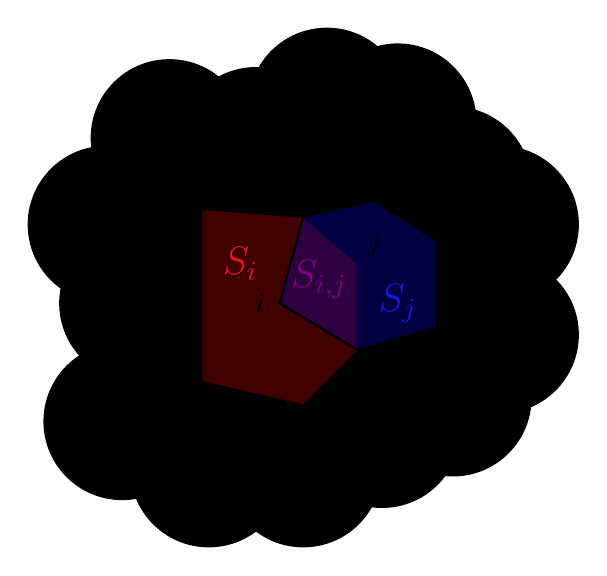
\begin{tikzpicture}[
  scale=1]

\coordinate (p1) at (1,1);
\coordinate (p2) at (2.1,0.4);
\coordinate (p3) at (3.3,0.4);
\coordinate (p4) at (4.3,0.9);
\coordinate (p5) at (5.2,1.3);
\coordinate (p6) at (5.8,2.1);
\coordinate (p7) at (5.8,3.5);
\coordinate (p8) at (5.2,4);
\coordinate (p9) at (4.5,4.8);
\coordinate (p10) at (3.6,5);
\coordinate (p11) at (2.7,4.5);
\coordinate (p12) at (1.6,4.6);
\coordinate (p13) at (0.8,3.5);
\coordinate (p14) at (1.2,2.5);
\coordinate (p15) at (2,1.5);
\coordinate (p16) at (3.3,1.2);
\coordinate (p17) at (4,1.9);
\coordinate (p18) at (5,2.2);
\coordinate (p19) at (5,3.3);
\coordinate (p20) at (4.2,3.8);
\coordinate (p21) at (3.3,3.6);
\coordinate (p22) at (2,3.7);
\coordinate (i) at (3,2.5);
\coordinate (j) at (4,3);

\fill (p1) circle (\pointsize);
\fill (p2) circle (\pointsize);
\fill (p3) circle (\pointsize);
\fill (p4) circle (\pointsize);
\fill (p5) circle (\pointsize);
\fill (p6) circle (\pointsize);
\fill (p7) circle (\pointsize);
\fill (p8) circle (\pointsize);
\fill (p9) circle (\pointsize);
\fill (p10) circle (\pointsize);
\fill (p11) circle (\pointsize);
\fill (p12) circle (\pointsize);
\fill (p13) circle (\pointsize);
\fill (p14) circle (\pointsize);
\fill (p15) circle (\pointsize);
\fill (p16) circle (\pointsize);
\fill (p17) circle (\pointsize);
\fill (p18) circle (\pointsize);
\fill (p19) circle (\pointsize);
\fill (p20) circle (\pointsize);
\fill (p21) circle (\pointsize);
\fill (p22) circle (\pointsize);
\fill (i) circle (\pointsize);
\fill (j) circle (\pointsize);

\draw (p1) -- (p2);
\draw (p1) -- (p14);
\draw (p1) -- (p15);
\draw (p2) -- (p3);
\draw (p2) -- (p15);
\draw (p2) -- (p16);
\draw (p3) -- (p4);
\draw (p3) -- (p16);
\draw (p4) -- (p5);
\draw (p4) -- (p16);
\draw (p4) -- (p17);
\draw (p4) -- (p18);
\draw (p5) -- (p6);
\draw (p5) -- (p18);
\draw (p6) -- (p7);
\draw (p6) -- (p18);
\draw (p6) -- (p19);
\draw (p7) -- (p8);
\draw (p7) -- (p19);
\draw (p8) -- (p9);
\draw (p8) -- (p19);
\draw (p8) -- (p20);
\draw (p9) -- (p10);
\draw (p9) -- (p20);
\draw (p10) -- (p11);
\draw (p10) -- (p20);
\draw (p10) -- (p21);
\draw (p11) -- (p12);
\draw (p11) -- (p21);
\draw (p11) -- (p22);
\draw (p12) -- (p13);
\draw (p12) -- (p22);
\draw (p13) -- (p14);
\draw (p13) -- (p22);
\draw (p14) -- (p15);
\draw (p14) -- (p22);
\draw (p15) -- (i);
\draw (p15) -- (p16);
\draw (p15) -- (p22);
\draw (p16) -- (i);
\draw (p16) -- (p17);
\draw (p17) -- (i);
\draw (p17) -- (j);
\draw (p17) -- (p18);
\draw (p18) -- (j);
\draw (p18) -- (p19);
\draw (p19) -- (j);
\draw (p19) -- (p20);
\draw (p20) -- (j);
\draw (p20) -- (p21);
\draw (p21) -- (i);
\draw (p21) -- (j);
\draw (p21) -- (p22);
\draw (p22) -- (i);
\draw (i) -- (j);

\draw[thick, draw=black, fill=red, fill opacity=0.25] (p15)--(p16)--(p17)--(j)
  --(p21)--(p22)--cycle;
\draw[thick, draw=black, fill=blue, fill opacity=0.25] (p17)--(p18)--(p19)--(p20)
  --(p21)--(i)--cycle;

\node at ($(i)-(0.25,0)$) {$i$};
\node at ($(j)+(0.2,0.25)$) {$j$};

\node at (2.5,3) {\Large $\textcolor{gray!20!red}{\support_i}$};
\node at (3.5,2.8) {\Large $\textcolor{violet}{\support\ij}$};
\node at (4.5,2.5) {\Large $\textcolor{gray!20!blue}{\support_j}$};

\end{tikzpicture}

\end{minipage}
\begin{minipage}{0.49\textwidth}
  \begin{itemize}
    \item Let \hlorange{$\indices(\cell)$} be the set of DoF indices on cell $\cell$.
    \item Let \hlorange{$n_\cell$} be the number of DoFs on cell $\cell$.
  \end{itemize}
  \begin{tikzpicture}[
  scale=1]

\input{content/diagrams/mesh.tex}

\draw[draw=none, fill=red, fill opacity=0.5] (p15)--(p16)--(p17)--(j)
  --(p21)--(p22)--cycle;
\draw[draw=none, fill=blue, fill opacity=0.5] (p17)--(p18)--(p19)--(p20)
  --(p21)--(i)--cycle;
\draw[draw=none, fill=yellow, fill opacity=0.5] (p16)--(i)--(j)--(p18)
  --(p4)--cycle;

\node[black] at ($0.333*(i) + 0.333*(j) + 0.333*(p17)$) {\Large $K$};

\fill[black] (i) circle (\pointsize);
\fill[black] (j) circle (\pointsize);
\fill[black] (p17) circle (\pointsize);

\end{tikzpicture}

\end{minipage}

\end{frame}
%%%%%%%%%%%%%%%%%%%%%%%%%%%%%%%%%%%%%%%%%%%%%%%%%%%%%%%%%%%%%%%%%%%%%%%%%%%%%%%%
\begin{frame}
\frametitle{Discretization}

\begin{itemize}
   \item Discretizing with forward Euler (FE) in time and \hlorange{Galerkin CFEM}
      in space gives
   \begin{equation}
      \consistentmassmatrix\frac{\solutionvector^{n+1}-\solutionvector^n}
        {\dt} + \ssmatrix\solutionvector^n = \ssrhs^n \eqc
   \end{equation}
   where
   \begin{equation}
     M\ij^C \equiv \int\limits_{\support\ij}
       \testfunction_i(\x) \testfunction_j(\x) d\x \eqc
   \end{equation}
   \begin{equation}
     A\ij \equiv \int\limits_{\support\ij}\left(
       \mathbf{v}\cdot\nabla\testfunction_j(\x) +
		\reactioncoef(\x)\testfunction_j(\x)\right)\testfunction_i(\x) d\x \eqc
   \end{equation}
   \begin{equation}
      b_i^n \equiv \int\limits_{S_i} q(\x,t^n)\testfunction_i(\x) d\x \eqp
   \end{equation}
\end{itemize}

\end{frame}
%%%%%%%%%%%%%%%%%%%%%%%%%%%%%%%%%%%%%%%%%%%%%%%%%%%%%%%%%%%%%%%%%%%%%%%%%%%%%%%%
\begin{frame}
\frametitle{Temporal Discretization}

\begin{itemize}
  \item \hlorange{Forward Euler (FE)}:
    \begin{equation}
      \consistentmassmatrix\frac{\solutionvector^{n+1}-\solutionvector^n}
        {\dt} + \ssmatrix\solutionvector^n = \ssrhs^n \eqc
    \end{equation}
  \item \hlorange{Strong Stability Preserving Runge-Kutta (SSPRK) Methods}:
    %\begin{itemize}
    %  \item Can be expressed as a combination of FE-like steps:
    %\end{itemize}
\begin{subequations}
\begin{align}
  & \RKstagesolution^0 = \solutionvector^n \\
%  & \RKstagesolution^i = \gamma_i \solutionvector^n + \zeta_i \sq{
%      \RKstagesolution^{i-1}
%      + \dt\mathbf{G}(t^n+c_i\dt, \RKstagesolution^{i-1})}
  & \RKstagesolution^i = \gamma_i \solutionvector^n + \zeta_i \bar{\solutionvector}^i
    \eqc \quad 
      \consistentmassmatrix\frac{\bar{\solutionvector}^i-\RKstagesolution^{i-1}}
        {\dt} + \ssmatrix\RKstagesolution^{i-1} = \ssrhs(t_i) \eqc
    %\eqc \quad
    %i = 1,\ldots,s \eqc
    \\
  & \solutionvector^{n+1} = \RKstagesolution^s
\end{align}
\end{subequations}
  where $t_i \equiv t^n+c_i\dt$, and $\{\gamma_i,\zeta_i,c_i\}_{i=1}^s$
  depend on the method.
  \item \hlorange{Theta Method}:
\begin{subequations}
\begin{equation}
  \consistentmassmatrix\frac{\solutionvector^{\timeindex+1}
    - \solutionvector^\timeindex}{\timestepsize}
    + \ssmatrix\solutionvector^\theta
    = \ssrhs^\theta
\end{equation}
\begin{equation}
  \solutionvector^\theta \equiv (1-\theta)\solutionvector^n
    + \theta\solutionvector^{n+1}
  \eqc \quad
  \ssrhs^\theta \equiv (1-\theta)\ssrhs^n
    + \theta\ssrhs^{n+1}
\end{equation}
\end{subequations}
    where $0\leq\theta\leq1$.
\end{itemize}

\end{frame}
%%%%%%%%%%%%%%%%%%%%%%%%%%%%%%%%%%%%%%%%%%%%%%%%%%%%%%%%%%%%%%%%%%%%%%%%%%%%%%%%
\subsection{Boundary Conditions}
%%%%%%%%%%%%%%%%%%%%%%%%%%%%%%%%%%%%%%%%%%%%%%%%%%%%%%%%%%%%%%%%%%%%%%%%%%%%%%%%
\begin{frame}
\frametitle{Boundary Conditions}

\begin{itemize}
  \item The following 3 methods for imposing incoming flux boundary conditions
    for node $i$ are considered:
    \begin{enumerate}
      \item \hlorange{Strongly impose}: \emph{replace} equation $i$ with the equation
        $U_i = u^{\textup{inc}}(\x_i)$.
      \item \hlorange{Weakly impose}: evaluate incoming boundary fluxes 
        in equation $i$ with values $u^{\textup{inc}}(\x_j)$ instead of values $U_j$.
      \item Weakly impose with \hlorange{boundary penalty}: \emph{add} to
        equation $i$ a multiple $\alpha_i$ of the equation $U_i = u^{\textup{inc}}(\x_i)$,
        where $\alpha_i$ should be large enough such that this \emph{penalty}
        equation dominates the original equation $i$.
    \end{enumerate}
  \item The choice of incoming flux boundary condition will later to
    be shown to have consequences on conservation for FCT.
\end{itemize}

\end{frame}

%%%%%%%%%%%%%%%%%%%%%%%%%%%%%%%%%%%%%%%%%%%%%%%%%%%%%%%%%%%%%%%%%%%%%%%%%%%%%%%%%
\subsection{Low-Order Scheme}
%%%%%%%%%%%%%%%%%%%%%%%%%%%%%%%%%%%%%%%%%%%%%%%%%%%%%%%%%%%%%%%%%%%%%%%%%%%%%%%%%
\begin{frame}
\frametitle{Low-Order Scheme}

\begin{itemize}
   \item To get the low-order scheme, one does the following:
   \begin{itemize}
      \item Lumps the mass matrix:
        $\consistentmassmatrix\rightarrow\lumpedmassmatrix$.
      \item Adds a low-order diffusion operator:
        $\ssmatrix \rightarrow \ssmatrix+\loworderdiffusionmatrix$.
   \end{itemize}
   \item This gives the following, where $\solutionvector^{L,n+1}$ is the
     low-order solution:
   \begin{equation}
      \textcolor{secondarycolorheavy}{\lumpedmassmatrix}
        \frac{\solutionvector^{L,n+1}-\solutionvector^n}{\dt}
        + (\ssmatrix + \textcolor{secondarycolorheavy}{\diffusionmatrix^L})
          \solutionvector^n = \ssrhs^n \eqp
   \end{equation}
   \item The diffusion matrix $\diffusionmatrix^L$ is assembled elementwise,
      where $K$ denotes an element, using a local bilinear form $b_K$ and a
      local low-order viscosity $\nu_K^L$:
   \begin{equation}
      D\ij^L = \sumKSij \nu_K^L b_K(\testfunction_j,\testfunction_i) \eqp
   \end{equation}
\end{itemize}

\end{frame}
%%%%%%%%%%%%%%%%%%%%%%%%%%%%%%%%%%%%%%%%%%%%%%%%%%%%%%%%%%%%%%%%%%%%%%%%%%%%%%%%%
\begin{frame}
\frametitle{Local Viscous Bilinear Form}

\begin{itemize}
   \item The local viscous bilinear form is defined as follows, where $V_K$ denotes
      the volume of element $K$:
   \begin{equation}
      b_K(\testfunction_j, \testfunction_i) \equiv \left\{\begin{array}{l l}
         -\frac{1}{n_K - 1}V_K & i\ne j, \quad i,j\in \mathcal{I}(K)\\
         V_K                   & i = j,  \quad i,j\in \mathcal{I}(K)\\
         0                & i\notin\mathcal{I}(K)\,|\, j\notin\mathcal{I}(K)
      \end{array}\right. \eqp
   \end{equation}
   \item Some properties that result from this definition are
   \begin{subequations}
   \begin{equation}
      b_K(\testfunction_i, \testfunction_i) > 0 \eqp
   \end{equation}
   \begin{equation}
      b_K(\testfunction_j, \testfunction_i) < 0 \quad j \ne i \eqp
   \end{equation}
   \begin{equation}
      \sum\limits_j b_K(\testfunction_j, \testfunction_i) = 0 \eqp
   \end{equation}
   \end{subequations}
  \item The local viscous matrix in 1-D is
    \begin{equation}
      \mathbf{D}_K = \left[\begin{array}{r r}
           1 & -1\\
          -1 &  1
        \end{array}\right]\Delta x \eqp
    \end{equation}
\end{itemize}

\end{frame}
%%%%%%%%%%%%%%%%%%%%%%%%%%%%%%%%%%%%%%%%%%%%%%%%%%%%%%%%%%%%%%%%%%%%%%%%%%%%%%%%%
\begin{frame}
\frametitle{Low-Order Viscosity}

\begin{itemize}
   \item The low-order viscosity is defined as
   \begin{equation}
     \lowordercellviscosity[\timeindex] \equiv \max\limits_{i\ne j\in\indices(\cell)}
     \frac{\max(0,\ssmatrixletter\ij^\timeindex)}
     {-\mkern-20mu\sumKSij[T]\mkern-20mu\localviscbilinearform{T}{j}{i}}
     \eqp
   \end{equation}
   \item This definition is designed to be the smallest number such that the
      following is guaranteed:
   \begin{equation}
      D^L\ij \leq -A\ij, \quad j\ne i \eqp
   \end{equation}
   \item This is used to guarantee that the low-order steady-state matrix
      $\ssmatrix^L=\ssmatrix+\diffusionmatrix^L$ is an M-matrix.
\end{itemize}

\end{frame}
%%%%%%%%%%%%%%%%%%%%%%%%%%%%%%%%%%%%%%%%%%%%%%%%%%%%%%%%%%%%%%%%%%%%%%%%%%%%%%%%%
\begin{frame}
\frametitle{M-Matrix Property}

\begin{itemize}
  \item An M-matrix, also known as a \hlorange{monotone matrix}, or
    \hlorange{inverse-positive matrix} has the property
    \begin{equation}
      \mathbf{A}\mathbf{x}=\mathbf{b} \ge 0\Rightarrow \mathbf{x}\ge 0 \eqp
    \end{equation}
  \item Therefore one can prove \hlorange{non-negativity} of the solution of
    a linear system $\mathbf{A}\solutionvector=\mathbf{b}$ by proving that
    $\mathbf{A}$ is an M-matrix and $\mathbf{b}$ is non-negative.
  \item An M-matrix can be identified by verifying the following properties:
    \begin{subequations}
      \begin{equation}
        A\ij \leq 0 \quad j \ne i \quad \forall i
      \end{equation}
      \begin{equation}
        A_{i,i} \geq 0 \quad \forall i
      \end{equation}
      \begin{equation}
        \sumj A\ij \geq 0 \quad \forall i
      \end{equation}
    \end{subequations}
\end{itemize}

\end{frame}
%%%%%%%%%%%%%%%%%%%%%%%%%%%%%%%%%%%%%%%%%%%%%%%%%%%%%%%%%%%%%%%%%%%%%%%%%%%%%%%%%
\begin{frame}
\frametitle{Local Discrete Maximum Principle for Explicit Euler}

\begin{itemize}
  \item If the following CFL-like condition is satisfied:
    \begin{equation}
      \dt \leq \frac{\massmatrixletter^L_{i,i}}{
        \ssmatrixletter_{i,i}^{L}}
      \quad\forall i \eqc
    \end{equation}
  then the low-order solution for explicit Euler satisfies the following
  \hlorange{local discrete maximum principle} (DMP):
      \begin{subequations}
      \begin{equation}
         \DMPlowerbound_i \leq
         U_i^{L,n+1}\leq
         \DMPupperbound_i \qquad\forall i \eqc
      \end{equation}
      \begin{equation}
         \DMPbounds_i \equiv U_{\substack{\max\\\min},i}^n\left(
         1-\frac{\dt}{M_{i,i}^L}
         \sum\limits_j A\ij^L\right)
         + \frac{\Delta t}{M_{i,i}^L}b_i^n \eqc
      \end{equation}
      \begin{equation}
        U^n_{\substack{\max\\\min},i}
          = \substack{\max\\\min\limits_{j\in\mathcal{I}(S_i)}} U^n_j \eqp
      \end{equation}
      \end{subequations}
%   \item For example, when there is no reaction term or source term, this reduces
%      to the following DMP, which implies the scheme is local extremum
%      diminishing (LED):
%      \begin{equation}
%         U^n_{\min,i}\leq
%         U_i^{L,n+1}\leq
%         U^n_{\max,i}\qquad\forall i \eqp
%      \end{equation}
\end{itemize}

\end{frame}
%%%%%%%%%%%%%%%%%%%%%%%%%%%%%%%%%%%%%%%%%%%%%%%%%%%%%%%%%%%%%%%%%%%%%%%%%%%%%%%%%
\begin{frame}
\frametitle{Local Discrete Maximum Principle for Theta Method}

\begin{itemize}
  \item If the following CFL-like condition is satisfied:
    \begin{equation}
      \dt \leq \frac{\massmatrixletter^L_{i,i}}{(1-\theta)
        \ssmatrixletter_{i,i}^{L}}
      \quad\forall i \eqc
    \end{equation}
   then the low-order theta method solution satisfies the following local DMP,
   which is \hlorange{implicit}:
\begin{subequations}
\begin{multline}
   \DMPbounds_i\hlorange{(\solutionvector^{L,n+1})}
   \equiv
   \frac{1}{1+\frac{\theta\timestepsize}{\massmatrixletter^L_{i,i}}
       \ssmatrixletter_{i,i}^{L}}
     \Bigg[\pr{1 - \frac{(1-\theta)\timestepsize}{\massmatrixletter^L_{i,i}}
     \ssmatrixletter_{i,i}^{L}}\solutionletter_i^\timeindex
     \\
     - \frac{\timestepsize}{\massmatrixletter^L_{i,i}}
       \sumjnoti\ssmatrixletter_{i,j}^{L}\pr{
         (1-\theta)\solutionletter_{\substack{\max\\\min},j\ne i}^n
         + \theta\hlorange{\solutionletter_{\substack{\max\\\min},j\ne i}^{L,n+1}}}
     + \frac{\timestepsize}{\massmatrixletter^L_{i,i}}
       \ssrhsletter_i^\theta\Bigg] \eqc
\end{multline}
\begin{equation}
  \solutionletter_{\substack{\max\\\min},j\ne i}^\timeindex
  \equiv \substack{\max\\\min\limits_{j\ne i\in\indices(\support_i)}}
    \solutionletter_j^\timeindex
  \eqp
\end{equation}
\end{subequations}
\end{itemize}

\end{frame}
%%%%%%%%%%%%%%%%%%%%%%%%%%%%%%%%%%%%%%%%%%%%%%%%%%%%%%%%%%%%%%%%%%%%%%%%%%%%%%%%%
\begin{frame}
\frametitle{Low-Order Scheme Results Example}
\framesubtitle{Linear Advection of Discontinuous Wave Front}

\begin{center}
\includegraphics[width=0.85\textwidth]{./figures/advection_low_order.pdf}
\end{center}

\end{frame}

\input{content/scalar_high}
%%%%%%%%%%%%%%%%%%%%%%%%%%%%%%%%%%%%%%%%%%%%%%%%%%%%%%%%%%%%%%%%%%%%%%%%%%%%%%%%%
\subsection{FCT Scheme}
%%%%%%%%%%%%%%%%%%%%%%%%%%%%%%%%%%%%%%%%%%%%%%%%%%%%%%%%%%%%%%%%%%%%%%%%%%%%%%%%%
\begin{frame}
\frametitle{FCT Antidiffusive Flux Definition}

\begin{itemize}
   \item Recall that FCT defines antidiffusive correction fluxes
      from a low-order, monotone scheme to a high-order scheme. Calling
      these fluxes $\correctionfluxvector$, this gives
      \begin{equation}
        \lumpedmassmatrix\frac{
          \textcolor{secondarycolorheavy}{\solutionvector^{H}}
            -\solutionvector^n}{\dt}
          + (\ssmatrix+\diffusionmatrix^L)\solutionvector^n = \ssrhs^n
          + \textcolor{secondarycolorheavy}{\correctionfluxvector} \eqp
      \end{equation}
   \item Subtracting the high-order scheme equation from this gives the
      definition of $\correctionfluxvector$:
      \begin{equation}
        \correctionfluxvector \equiv
          -(\consistentmassmatrix-\lumpedmassmatrix)
          \frac{\solutionvector^{H}-\solutionvector^n}{\dt}
          + (\diffusionmatrix^L-\diffusionmatrix^{H,n})\solutionvector^n \eqp
      \end{equation}
   \item Decomposing $\correctionfluxvector$ into internodal fluxes
      $\correctionfluxij$ such that $\sum_j \correctionfluxij =
      \correctionfluxletter_i$,
   \begin{equation}
     \correctionfluxij = -M\ij^C\pr{
       \frac{\solutionletter^{H}_j-\solutionletter^n_j}{\Delta t}
       -\frac{\solutionletter^{H}_i-\solutionletter^n_i}{\Delta t}
       }
       + (D\ij^L-D\ij^{H,n})\pr{\solutionletter^n_j-\solutionletter^n_i} \eqp
   \end{equation}
\end{itemize}

\end{frame}
%%%%%%%%%%%%%%%%%%%%%%%%%%%%%%%%%%%%%%%%%%%%%%%%%%%%%%%%%%%%%%%%%%%%%%%%%%%%%%%%%
\begin{frame}
\frametitle{FCT Scheme Overview}

\begin{itemize}
   \item Recall that the objective of FCT is to limit these antidiffusive
      fluxes to enforce some physical solution bounds:
      \begin{equation}
         W_i^-\leq
         U_i^{n+1}\leq
         W_i^+\qquad\forall i \eqc
      \end{equation}
      for example, the low-order DMP bounds.
   \item This is achieved by applying a limiting coefficient \hlorange{$L\ij$} to each
      antidiffusion flux $\correctionfluxij$:
      \begin{equation}
        \lumpedmassmatrix\frac{\solutionvector^{n+1}-\solutionvector^n}{\dt}
          + \ssmatrix^L\solutionvector^n = \ssrhs
          + \hlorange{\bar{\correctionfluxvector}} \eqc
      \end{equation}
      where $\bar{\correctionfluxletter}_i \equiv \sumj\hlorange{L\ij}\correctionfluxij$.
   \item Each limiting coefficient is between zero and unity:
     \hlorange{$0\leq L\ij\leq 1$}.
   \begin{itemize}
      \item If all $L\ij$ are zero, then the low-order scheme is produced.
      \item If all $L\ij$ are one, then the high-order scheme is produced.
   \end{itemize}
\end{itemize}

\end{frame}
%%%%%%%%%%%%%%%%%%%%%%%%%%%%%%%%%%%%%%%%%%%%%%%%%%%%%%%%%%%%%%%%%%%%%%%%%%%%%%%%%
\begin{frame}
\frametitle{Conservation}

\begin{itemize}
  \item FCT scheme is \hlorange{conservative} if the net antidiffusion source
    is zero:
    \begin{equation}
      \sum\limits_i \bar{\correctionfluxletter}_i
        = \sum\limits_i\sumj L\ij\correctionfluxij = 0 \eqp
    \end{equation}
  \item The antidiffusive flux decomposition choice yielded
    $\correctionfluxji = -\correctionfluxij$ and $\correctionfluxentry_{i,i}=0$.
    Therefore $\sum_i\sum_j\correctionfluxij = 0$.
  \item Then if one enforces symmetry on the limiting coefficients, then
    conservation is achieved:
    \begin{equation}
      L\ji = L\ij \quad \Rightarrow \quad
      \sum\limits_i \bar{\correctionfluxletter}_i = 0 \eqp
    \end{equation}
  \item \hlorange{Caveat}: When Dirichlet BC are \emph{strongly} imposed, the FCT
    scheme is not conservative unless all antidiffusive fluxes from Dirichlet
    nodes are completely cancelled.
    \begin{itemize}
      \item The flux decomposition is incorrect in the vicinity of Dirichlet nodes.
      \item Equations for Dirichlet nodes overwrite contribution from antidiffusion
        sources.
    \end{itemize}
\end{itemize}

\end{frame}
%%%%%%%%%%%%%%%%%%%%%%%%%%%%%%%%%%%%%%%%%%%%%%%%%%%%%%%%%%%%%%%%%%%%%%%%%%%%%%%%%
\begin{frame}
\frametitle{Antidiffusion Bounds}

\begin{itemize}
   \item The solution bounds translate to antidiffusion bounds:
      \begin{equation}
         W_i^-\leq
         U_i^{n+1}\leq
         W_i^+
         \quad \Rightarrow \quad
         Q^-_i \leq \bar{\correctionfluxletter}_i \leq Q^+_i \eqp
      \end{equation}
   \item For explicit Euler, $Q_i^\pm$ is found to be
      \begin{equation}
         Q_i^\pm \equiv M_{i,i}^L\frac{W_i^\pm-U_i^n}{\Delta t}
         + \sum\limits_j A_{i,j}^L U_j^n - b_i^n \eqp
      \end{equation}
  \item Most limiters assume
    \begin{equation}
      Q_i^+ \geq 0  \eqc \quad Q_i^- \leq 0 \quad \forall i \eqp
    \end{equation}
    \begin{itemize}
      \item FCT starts from low-order solution:
        $\bar{\correctionfluxletter}_i = 0 \quad \Rightarrow \quad
          \solutionletter^{FCT}_i = \solutionletter^L_i$.
      \item Some solution bounds automatically satisfy these requirements;
        otherwise one must enforce them:
        \begin{equation}
          Q_i^+ \gets \max(0,Q_i^+) \eqc \quad Q_i^- \gets \min(0,Q_i^-) \eqp
        \end{equation}
    \end{itemize}
\end{itemize}

\end{frame}
%%%%%%%%%%%%%%%%%%%%%%%%%%%%%%%%%%%%%%%%%%%%%%%%%%%%%%%%%%%%%%%%%%%%%%%%%%%%%%%%%
\begin{frame}
\frametitle{Limiters}

\begin{itemize}
  \item The objective of an FCT limiter is to \hlorange{maximize antidiffusion
    without violating imposed solution bounds}:

    \begin{quote}
      Find $0\leq \{L\ij\} \leq 1$ such that
      $\sum_i\bar{\correctionfluxletter}_i$ is maximized, subject
      to the constraints $Q_i^-\leq \bar{\correctionfluxletter}_i\leq Q_i^+$,
      $\forall i$.
    \end{quote}
  \item Zalesak's limiter is the following:
      \begin{subequations}
      \begin{equation}
         L\ij \equiv\left\{
            \begin{array}{l l}
               \min(L_i^+,L_j^-) & \correctionfluxij \geq 0\\
               \min(L_i^-,L_j^+) & \correctionfluxij < 0
            \end{array}
            \right. \eqc
      \end{equation}
      \begin{equation}
         L_i^\pm \equiv\left\{
            \begin{array}{l l}
               1 & \correctionfluxletter_i^\pm = 0\\
               \min\left(1,\frac{Q_i^\pm}{\correctionfluxletter_i^\pm}\right) &
                 \correctionfluxletter_i^\pm \ne 0
            \end{array}
            \right. \eqc
      \end{equation}
      \begin{equation}
        \correctionfluxletter_i^- \equiv \sum\limits_{j:\correctionfluxij<0}
          \correctionfluxij \eqc \qquad
        \correctionfluxletter_i^+ \equiv \sum\limits_{j:\correctionfluxij>0}
          \correctionfluxij \eqp
      \end{equation}
      \end{subequations}
\end{itemize}

\end{frame}
%%%%%%%%%%%%%%%%%%%%%%%%%%%%%%%%%%%%%%%%%%%%%%%%%%%%%%%%%%%%%%%%%%%%%%%%%%%%%%%%%
\begin{frame}
\frametitle{FCT Scheme Results Example}
\framesubtitle{Linear Advection of Discontinuous Wave Front}

\includegraphics[width=\textwidth]{./figures/advection_FCT.pdf}

\end{frame}
%%%%%%%%%%%%%%%%%%%%%%%%%%%%%%%%%%%%%%%%%%%%%%%%%%%%%%%%%%%%%%%%%%%%%%%%%%%%%%%%%
\begin{frame}
\frametitle{Analytic Solution Bounds}

\begin{itemize}
  \item Solution bounds can be derived using the
    \hlorange{method of characteristics} (MoC):
  \begin{subequations}
  \begin{equation}
      W_i^{\textup{MoC},+}
        \equiv
          \solutionletter_{\max,i}^n
            e^{-\dt\reactioncoef_{\min,i}}
            + \frac{\scalarsource_{\max,i}}
              {\reactioncoef_{\min,i}}
            (1 - e^{-\dt\reactioncoef_{\min,i}}) \eqc
  \end{equation}
  \begin{equation}
      W_i^{\textup{MoC},-}
        \equiv
          \solutionletter_{\min,i}^n
            e^{-\dt\reactioncoef_{\max,i}}
            + \frac{\scalarsource_{\min,i}}
              {\reactioncoef_{\max,i}}
            (1 - e^{-\dt\reactioncoef_{\max,i}}) \eqp
  \end{equation}
  \begin{equation}
    \reactioncoef_{\max,i} = \max\limits_{\x\in\support_i}\reactioncoef(\x) \eqc
    \quad \scalarsource_{\max,i} = \max\limits_{\x\in\support_i}\scalarsource(\x) \eqc
  \end{equation}
  \end{subequations}
  \item Recall the low-order DMP bounds for explicit Euler:
  \begin{subequations}
      \begin{equation}
         \DMPbounds_i \equiv U_{\substack{\max\\\min},i}^n\left(
         1-\dt\bar{\reactioncoef}_i\right)
         + \dt\bar{\scalarsource}_i \eqc
      \end{equation}
      \begin{equation}
        \bar{\reactioncoef}_i \equiv
          \frac{\intSi\reactioncoef\testfunction_i\dvolume}
            {\intSi\testfunction_i\dvolume}
        \eqc \quad
        \bar{\scalarsource}_i \equiv
          \frac{\intSi\scalarsource\testfunction_i\dvolume}
            {\intSi\testfunction_i\dvolume}
      \end{equation}
  \end{subequations}
\end{itemize}

\end{frame}

In this research, implicit and steady-state temporal discretizations are
considered for the scalar case only. The examples given in this section thus
correspond to the scalar case; however, the same methodology could be used
for systems of conservation laws.

The nonlinear systems considered in this research can be written in a quasilinear
form:
\begin{equation}\label{eq:nonlinear_equation}
  \nonlinearmatrix(\solutionvector)\solutionvector
    = \nonlinearrhs(\solutionvector) \eqp
\end{equation}
The right-hand-side $\nonlinearrhs(\solutionvector)$ is a function of
the solution for FCT schemes since in general the limiting coefficients are
functions of the solution.
A system in which Dirichlet boundary conditions are strongly imposed
requires modification of the matrix and right-hand-side vector:
$\nonlinearmatrix\rightarrow\dirichlet{\nonlinearmatrix}$ and
$\nonlinearrhs\rightarrow\dirichlet{\nonlinearrhs}$. In the remainder of
this section, the Dirichlet-modified notation is used to be general;
if strong Dirichlet boundary conditions are not applied, then the
Dirichlet-modified notation can simply be ignored. Subsequent sections
will define the matrix $\nonlinearmatrix$ and $\nonlinearrhs$ for different
nonlinear schemes.

To solve this system, fixed point iteration will be used:
\begin{equation}
  \dirichlet{\nonlinearmatrix}^{(\ell)}\solutionvector^{(\ell+1)}
    = \dirichlet{\nonlinearrhs}^{(\ell)} \eqc
\end{equation}
where $\nonlinearmatrix^{(\ell)}\equiv\nonlinearmatrix(\solutionvector^{(\ell)})$
and $\nonlinearrhs^{(\ell)}\equiv\nonlinearrhs(\solutionvector^{(\ell)})$.
However, in implementation, this will be expressed as a defect correction scheme:
\begin{equation}
  \ssres^{(\ell)} = \dirichlet{\nonlinearrhs}^{(\ell)}
    - \dirichlet{\nonlinearmatrix}^{(\ell)}\solutionvector^{(\ell)} \eqc
\end{equation}
\begin{equation}
  \dirichlet{\nonlinearmatrix}^{(\ell)}\Delta\solutionvector^{(\ell+1)}
    = \ssres^{(\ell)} \eqc
\end{equation}
\begin{equation}
  \solutionvector^{(\ell+1)} = \solutionvector^{(\ell)}
    + \Delta\solutionvector^{(\ell+1)} \eqp
\end{equation}
There are a number of advantages to this approach. Firstly this approach uses
the linear residual $\ssres^{(\ell)}$, which is advantageous when checking
for convergence; for example, there are a number of caveats associated with
checking convergence based on some measure of the difference between solution
iterates $\solutionvector^{(\ell)}$ and $\solutionvector^{(\ell+1)}$.

Another advantage of the defect correction approach is the ease in implementing
a relaxation parameter $\relaxationparameter$:
\begin{equation}
  \solutionvector^{(\ell+1)} = \solutionvector^{(\ell)}
    + \relaxationparameter\Delta\solutionvector^{(\ell+1)} \eqp
\end{equation}

The pseudocode for this defect correction scheme is given in Algorithm
\ref{alg:defect_correction}.
The notation $\|\ssres\|_X$ denotes some norm $X$ of $\ssres$.
The initial guess is denoted by $\solutionvector^{\text{guess}}$. For
transient calculations, the previous time step solution $\solutionvector^n$
is often used as the guess, and for steady-state calculations, one
could use a zero vector as the initial guess.

\begin{algorithm}[H]
\caption{Defect Correction Algorithm}
\label{alg:defect_correction}
\begin{algorithmic}
\State $\solutionvector^{(0)} \gets \solutionvector^{\text{guess}}$
\State \texttt{converged} $\gets$ \texttt{FALSE}
\For{$\ell\gets 0, \ell_{\text{max}}$}
  \State $\nonlinearmatrix^{(\ell)} \gets
    \nonlinearmatrix(\solutionvector^{(\ell)})$
  \State $\nonlinearrhs^{(\ell)} \gets
    \nonlinearrhs(\solutionvector^{(\ell)})$
  \State $\nonlinearmatrix^{(\ell)} \rightarrow \dirichlet{\nonlinearmatrix}^{(\ell)}$,
    $\nonlinearrhs^{(\ell)} \rightarrow \dirichlet{\nonlinearrhs}^{(\ell)}$,
  \State $\ssres^{(\ell)} \gets \dirichlet{\nonlinearrhs}^{(\ell)}
    - \dirichlet{\nonlinearmatrix}^{(\ell)}\solutionvector^{(\ell)}$
  \If{$\|\ssres^{(\ell)}\|_X < \nonlineartolerance$}
    \State \texttt{converged} $\gets$ \texttt{TRUE}
    \Break
  \EndIf
  \State $\Delta\solutionvector^{(\ell+1)}
    \gets \sq{\dirichlet{\nonlinearmatrix}^{(\ell)}}^{-1}\ssres^{(\ell)}$
  \State $\solutionvector^{(\ell+1)} \gets \solutionvector^{(\ell)}
    + \relaxationparameter\Delta\solutionvector^{(\ell+1)}$
\EndFor
\If{\Not \texttt{converged}}
  \Error{Solution did not converge within $\ell_{\text{max}}$ iterations}
\EndIf
\end{algorithmic}
\end{algorithm}

Table \ref{tab:nonlinear_systems} gives the definitions of the system matrix
and right-hand-side vector given by Equation \eqref{eq:nonlinear_equation}
for a number of different nonlinear schemes. These schemes include schemes
that use entropy viscosity and those that use FCT. For the equations of
transient schemes, the solution vector $\solutionvector^{n+1}$ uses
$\solutionvector$ as its notation; the superscript $n+1$ is understood.
This is to be consistent
with the convention that $\solutionvector$ is the vector iterated upon in
the nonlinear scheme.

Note that in Table \ref{tab:nonlinear_systems}, the low-order steady-state
matrix $\loworderssmatrix$ is assumed to be independent of the solution. This
is true for conservation laws with \emph{linear} conservation law flux
functions $\consfluxscalar$. For nonlinear $\consfluxscalar$, this is not the
case, and the nonlinear system matrix $\nonlinearmatrix$ for the FCT schemes
given in the table becomes a function of the solution and thus must be
recomputed in each iteration.

%-------------------------------------------------------------------------------
\begin{table}[htb]\caption{Nonlinear System Matrix and Right-hand-side Vector for
  Different Schemes}
\label{tab:nonlinear_systems}
\centering
\begin{tabular}{l p{4in}}\toprule
\multicolumn{2}{l}{\emph{Steady-State Entropy Viscosity Scheme}}\\\midrule
Equation &
  \parbox{4in}{\begin{equation*}
    \highorderssmatrix(\solutionvector)\solutionvector = \ssrhs
  \end{equation*}}\\
Matrix &
  \parbox{4in}{\begin{equation*}
    \nonlinearmatrix(\solutionvector)
      \equiv \highorderssmatrix(\solutionvector)
  \end{equation*}}\\
Right-hand-side &
  \parbox{4in}{\begin{equation*}
    \nonlinearrhs \equiv \ssrhs
  \end{equation*}}\\
\midrule
\multicolumn{2}{l}{\emph{Steady-State FCT Scheme}}\\\midrule
Equation &
  \parbox{4in}{\begin{equation*}
    \loworderssmatrix\solutionvector = \ssrhs
    + \limitermatrix(\solutionvector)\cdot\correctionfluxmatrix
  \end{equation*}}\\
Matrix &
  \parbox{4in}{\begin{equation*}
    \nonlinearmatrix \equiv \loworderssmatrix
  \end{equation*}}\\
Right-hand-side &
  \parbox{4in}{\begin{equation*}
    \nonlinearrhs(\solutionvector) \equiv \ssrhs
    + \limitermatrix(\solutionvector)\cdot\correctionfluxmatrix
  \end{equation*}}\\
\midrule
\multicolumn{2}{l}{\emph{Theta Entropy Viscosity Scheme}}\\\midrule
&\\[-5ex]
Equation &
  \parbox{4in}{\begin{multline*}
    \consistentmassmatrix\frac{\solutionvector-\solutionvector^n}{\dt}
    + (1-\theta)\ssmatrix^{H,n}\solutionvector^n
    + \theta\ssmatrix^{H}(\solutionvector)\solutionvector
    = \\[-1ex]
    (1-\theta)\ssrhs^n + \theta\ssrhs^{n+1}
  \end{multline*}}\\[-2ex]
Matrix &
  \parbox{4in}{\begin{equation*}
    \nonlinearmatrix(\solutionvector) \equiv \consistentmassmatrix
    + \theta\dt\ssmatrix^H(\solutionvector)
  \end{equation*}}\\[-2ex]
Right-hand-side &
  \parbox{4in}{\begin{multline*}
    \nonlinearrhs \equiv
      \consistentmassmatrix\solutionvector^n
      - (1-\theta)\dt\ssmatrix^{H,n}\solutionvector^n
      \\
      + (1-\theta)\dt\ssrhs^n + \theta\dt\ssrhs^{n+1}
  \end{multline*}}\\[-2ex]
\midrule
\multicolumn{2}{l}{\emph{Theta FCT Scheme}}\\\midrule
&\\[-5ex]
Equation &
  \parbox{4in}{\begin{multline*}
    \lumpedmassmatrix\frac{\solutionvector-\solutionvector^n}{\dt}
    + (1-\theta)\loworderssmatrix\solutionvector^{n}
    + \theta\loworderssmatrix\solutionvector
    = \\
    (1-\theta)\ssrhs^n + \theta\ssrhs^{n+1}
    + \limitermatrix(\solutionvector)\cdot\correctionfluxmatrix
  \end{multline*}}\\[-2ex]
Matrix &
  \parbox{4in}{\begin{equation*}
    \nonlinearmatrix \equiv \lumpedmassmatrix
    + \theta\dt\loworderssmatrix
  \end{equation*}}\\[-3ex]
Right-hand-side &
  \parbox{4in}{\begin{multline*}
    \nonlinearrhs(\solutionvector) \equiv
      \lumpedmassmatrix\solutionvector^n
      - (1-\theta)\dt\loworderssmatrix\solutionvector^n
      \\
      + (1-\theta)\dt\ssrhs^n + \theta\dt\ssrhs^{n+1}
      + \dt\limitermatrix(\solutionvector)\cdot\correctionfluxmatrix
  \end{multline*}}\\[-2ex]
\bottomrule\end{tabular}
\end{table}
%-------------------------------------------------------------------------------


%%%%%%%%%%%%%%%%%%%%%%%%%%%%%%%%%%%%%%%%%%%%%%%%%%%%%%%%%%%%%%%%%%%%%%%%%%%%%%%%%
\section{Scalar Results}
%%%%%%%%%%%%%%%%%%%%%%%%%%%%%%%%%%%%%%%%%%%%%%%%%%%%%%%%%%%%%%%%%%%%%%%%%%%%%%%%%
\begin{frame}
\frametitle{Source-in-Absorber Test Problem}
\framesubtitle{Strong Absorber with Source in Left Half of Domain, FE}

\begin{center}
\includegraphics[height=0.8\textheight]{./figures/solutions_source_FE.pdf}
\end{center}

\end{frame}
%%%%%%%%%%%%%%%%%%%%%%%%%%%%%%%%%%%%%%%%%%%%%%%%%%%%%%%%%%%%%%%%%%%%%%%%%%%%%%%%%
\begin{frame}
\frametitle{2-D Void-to-Absorber Test Problem}
\framesubtitle{Normally-Incident Wave from Void to Absorber Quadrant, FE}

\begin{figure}[h]
   \centering
   \begin{subfigure}{0.3\textwidth}
      \centering
      \includegraphics[width=0.8\textwidth]{./figures/exact.png}
      \caption{Exact}
   \end{subfigure}
   \begin{subfigure}{0.3\textwidth}
      \centering
      \includegraphics[width=0.8\textwidth]{./figures/Gal.png}
      \caption{Galerkin}
   \end{subfigure}
   \begin{subfigure}{0.3\textwidth}
      \centering
      \includegraphics[width=0.8\textwidth]{./figures/GalFCT.png}
      \caption{Galerkin-FCT}
   \end{subfigure}
   \begin{subfigure}{0.3\textwidth}
      \centering
      \includegraphics[width=0.8\textwidth]{./figures/low.png}
      \caption{Low-order}
   \end{subfigure}
   \begin{subfigure}{0.3\textwidth}
      \centering
      \includegraphics[width=0.8\textwidth]{./figures/EV.png}
      \caption{EV}
   \end{subfigure}
   \begin{subfigure}{0.3\textwidth}
      \centering
      \includegraphics[width=0.8\textwidth]{./figures/EVFCT.png}
      \caption{EV-FCT}
   \end{subfigure}
\end{figure}

\end{frame}
%%%%%%%%%%%%%%%%%%%%%%%%%%%%%%%%%%%%%%%%%%%%%%%%%%%%%%%%%%%%%%%%%%%%%%%%%%%%%%%%%
\begin{frame}
\frametitle{1-D Smooth Problem Convergence Test}
\framesubtitle{MMS Solution: $u(x,t)=t\sin(\pi x)$, FE}

\begin{center}
\includegraphics[height=0.8\textheight]{./figures/convergence_smooth_FE.pdf}
\end{center}

\end{frame}
%%%%%%%%%%%%%%%%%%%%%%%%%%%%%%%%%%%%%%%%%%%%%%%%%%%%%%%%%%%%%%%%%%%%%%%%%%%%%%%%%
\begin{frame}
\frametitle{1-D Non-smooth Problem Convergence Test}
\framesubtitle{Linear Advection of Discontinuous Wave Front, SSPRK33}

\begin{center}
\includegraphics[height=0.8\textheight]{./figures/convergence_absorber_SSPRK33.pdf}
\end{center}

\end{frame}
%%%%%%%%%%%%%%%%%%%%%%%%%%%%%%%%%%%%%%%%%%%%%%%%%%%%%%%%%%%%%%%%%%%%%%%%%%%%%%%%%
\begin{frame}
\frametitle{Obstruction Test Problem}
\framesubtitle{$45^\circ$-degree Flux Incident on Square Absorber Region, 4096 cells, FE}

\begin{figure}[h]
   \centering
   \begin{subfigure}{0.49\textwidth}
      \centering
      \includegraphics[width=\textwidth]{./figures/obstruction_Low_FE.png}
      \caption{Low-order}
   \end{subfigure}
   \begin{subfigure}{0.49\textwidth}
      \centering
      \includegraphics[width=\textwidth]{./figures/obstruction_EVFCT_FE.png}
      \caption{EV-FCT}
   \end{subfigure}
\end{figure}

\end{frame}
%%%%%%%%%%%%%%%%%%%%%%%%%%%%%%%%%%%%%%%%%%%%%%%%%%%%%%%%%%%%%%%%%%%%%%%%%%%%%%%%%
\begin{frame}
\frametitle{Obstruction Test Problem}
\framesubtitle{CFL Number vs. Iterations Study, Backward Euler, 256 cells}

\begin{center}
\begin{table}[h]
\caption{EV and FCT Iterations Required for EV-FCT Solution}
\begin{tabular}{c c c c c}\toprule
\emph{CFL} & \multicolumn{2}{c}{\emph{EV}} & \multicolumn{2}{c}{\emph{FCT}}\\
           & \emph{Total} & \emph{Avg.}    &  \emph{Total} & \emph{Avg.}\\\midrule
0.1  & 3999 &  8.14 & 3585 &   7.30\\
0.5  &  896 &  9.05 & 1499 &  15.14\\
1.0  &  501 & 10.02 &  970 &  19.40\\
5.0  &  157 & 15.70 & 1130 & 113.00\\
10.0 &   79 & 15.80 &  753 & 150.60\\
20.0 &   -- &    -- & \multicolumn{2}{c}{\textcolor{red}{\textbf{FAIL}}}\\
\bottomrule\end{tabular}
\end{table}
\end{center}

\end{frame}
%%%%%%%%%%%%%%%%%%%%%%%%%%%%%%%%%%%%%%%%%%%%%%%%%%%%%%%%%%%%%%%%%%%%%%%%%%%%%%%%%
\begin{frame}
\frametitle{Glance-in-Void Test Problem}
\framesubtitle{Glancing Incident Flux in a Vacuum, 4096 cells}

\begin{figure}[h]
   \centering
   \begin{subfigure}{0.3\textwidth}
      \centering
      \includegraphics[width=0.8\textwidth]{./figures/glance_DMP_FE.png}
      \caption{Low-order, FE}
   \end{subfigure}
   \begin{subfigure}{0.3\textwidth}
      \centering
      \includegraphics[width=0.8\textwidth]{./figures/glance_GalFCT_FE.png}
      \caption{Gal-FCT, FE}
   \end{subfigure}
   \begin{subfigure}{0.3\textwidth}
      \centering
      \includegraphics[width=0.8\textwidth]{./figures/glance_GalFCT_SSP3.png}
      \caption{Gal-FCT, SSPRK33}
   \end{subfigure}
   \begin{subfigure}{0.3\textwidth}
      \centering
      \includegraphics[width=0.8\textwidth]{./figures/glance_EV_FE_cE01.png}
      \caption{EV, FE}
   \end{subfigure}
   \begin{subfigure}{0.3\textwidth}
      \centering
      \includegraphics[width=0.8\textwidth]{./figures/glance_EVFCT_FE_cE01.png}
      \caption{EV-FCT, FE}
   \end{subfigure}
   \begin{subfigure}{0.3\textwidth}
      \centering
      \includegraphics[width=0.8\textwidth]{./figures/glance_EVFCT_SSP3_cE01.png}
      \caption{EV-FCT, SSPRK33}
   \end{subfigure}
\end{figure}

\end{frame}
%%%%%%%%%%%%%%%%%%%%%%%%%%%%%%%%%%%%%%%%%%%%%%%%%%%%%%%%%%%%%%%%%%%%%%%%%%%%%%%%%
\begin{frame}
\frametitle{Source-Void-to-Absorber Test Problem}
\framesubtitle{Strongly Imposed Dirichlet BC, $L^+=L^-=1$, SS}

\begin{center}
\includegraphics[height=0.8\textheight]{./figures/sourcevoid_strong1.pdf}
\end{center}

\end{frame}
%%%%%%%%%%%%%%%%%%%%%%%%%%%%%%%%%%%%%%%%%%%%%%%%%%%%%%%%%%%%%%%%%%%%%%%%%%%%%%%%%
\begin{frame}
\frametitle{Source-Void-to-Absorber Test Problem}
\framesubtitle{Strongly Imposed Dirichlet BC, $L^+=L^-=0$, SS}

\begin{center}
\includegraphics[height=0.8\textheight]{./figures/sourcevoid_strong0.pdf}
\end{center}

\end{frame}
%%%%%%%%%%%%%%%%%%%%%%%%%%%%%%%%%%%%%%%%%%%%%%%%%%%%%%%%%%%%%%%%%%%%%%%%%%%%%%%%%
\begin{frame}
\frametitle{Source-Void-to-Absorber Test Problem}
\framesubtitle{Weakly Imposed Dirichlet BC, SS}

\begin{center}
\includegraphics[height=0.8\textheight]{./figures/sourcevoid_weak.pdf}
\end{center}

\end{frame}
%%%%%%%%%%%%%%%%%%%%%%%%%%%%%%%%%%%%%%%%%%%%%%%%%%%%%%%%%%%%%%%%%%%%%%%%%%%%%%%%%
\begin{frame}
\frametitle{Source-Void-to-Absorber Test Problem}
\framesubtitle{Weakly Imposed Dirichlet BC With Boundary Penalty, SS}

\begin{center}
\includegraphics[height=0.8\textheight]{./figures/sourcevoid_penalty.pdf}
\end{center}

\end{frame}
%%%%%%%%%%%%%%%%%%%%%%%%%%%%%%%%%%%%%%%%%%%%%%%%%%%%%%%%%%%%%%%%%%%%%%%%%%%%%%%%%
\begin{frame}
\frametitle{Source-Void-to-Absorber Test Problem}
\framesubtitle{Number of Cells vs. Iterations Study, Backward Euler, CFL = 1}

\begin{center}
\begin{table}[h]
\caption{EV and FCT Iterations Required for EV-FCT Solution}
\begin{tabular}{c c c c c}\toprule
$N_{cell}$ & \multicolumn{2}{c}{\emph{EV}} & \multicolumn{2}{c}{\emph{FCT}}\\
           & \emph{Total} & \emph{Avg.}    &  \emph{Total} & \emph{Avg.}\\\midrule
  8 &  661 & 24.48 &   244 &  9.04\\
 16 &  807 & 19.21 &   655 & 15.60\\
 32 &  844 & 11.25 &  1194 & 15.92\\
 64 & 1204 &  8.72 &  2024 & 14.67\\
128 & 1752 &  6.59 &  3675 & 13.82\\
256 & 2713 &  5.20 &  6673 & 12.78\\
512 & 4284 &  4.14 & 12098 & 11.69\\
\bottomrule\end{tabular}
\end{table}
\end{center}

\end{frame}
%%%%%%%%%%%%%%%%%%%%%%%%%%%%%%%%%%%%%%%%%%%%%%%%%%%%%%%%%%%%%%%%%%%%%%%%%%%%%%%%%
\begin{frame}
\frametitle{Source-Void-to-Absorber Test Problem}
\framesubtitle{CFL Number vs. Iterations Study, Backward Euler, 128 cells}

\begin{center}
\begin{table}[h]
\caption{EV and FCT Iterations Required for EV-FCT Solution}
\begin{tabular}{c c c c c c c }\toprule
 & & \multicolumn{2}{c}{\emph{EV}}
  & \multicolumn{2}{c}{\emph{FCT}} &\\
\emph{CFL} & $N_{step}$ & \emph{Total} & \emph{Avg.}
  & \emph{Total} & \emph{Avg.} & $L^2$ \emph{err.}\\\midrule
0.1 & 2661 & 15006 &  5.64 & 14036 &   5.27 & $3.013\times10^{-3}$\\
0.5 &  533 &  3445 &  6.46 &  5000 &   9.38 & $3.033\times10^{-3}$\\
1.0 &  266 &  1752 &  6.59 &  3675 &  13.82 & $3.023\times10^{-3}$\\
5.0 &   54 &   471 &  8.72 & 12208 & 226.07 & $2.979\times10^{-3}$\\
10.0 &  27 &   232 &  8.59 &  6126 & 226.89 & $3.325\times10^{-3}$\\
20.0 &  14 &   133 &  9.50 &  3713 & 265.21 & $3.727\times10^{-3}$\\
50.0 &   6 &    62 & 10.33 &  2077 & 346.17 & $7.191\times10^{-3}$\\
\bottomrule\end{tabular}
\end{table}
\end{center}

\end{frame}


%%%%%%%%%%%%%%%%%%%%%%%%%%%%%%%%%%%%%%%%%%%%%%%%%%%%%%%%%%%%%%%%%%%%%%%%%%%%%%%%%
\section{Systems Methodology}
%%%%%%%%%%%%%%%%%%%%%%%%%%%%%%%%%%%%%%%%%%%%%%%%%%%%%%%%%%%%%%%%%%%%%%%%%%%%%%%%%
\subsection{Discretization}
%%%%%%%%%%%%%%%%%%%%%%%%%%%%%%%%%%%%%%%%%%%%%%%%%%%%%%%%%%%%%%%%%%%%%%%%%%%%%%%%%
\begin{frame}
\begin{center}
  \Huge{\textcolor{myblue}{The Shallow Water Equations}}
\end{center}
\end{frame}
%%%%%%%%%%%%%%%%%%%%%%%%%%%%%%%%%%%%%%%%%%%%%%%%%%%%%%%%%%%%%%%%%%%%%%%%%%%%%%%%%
\begin{frame}
\frametitle{Discretization}

\begin{itemize}
  \item A general system of conservation laws, with sources, is
    \begin{equation}
      \pd{\vectorsolution}{t} + \divergence\consfluxvector(\vectorsolution)
        = \conssource(\vectorsolution) \eqp
    \end{equation}
  \item After doing the following:
    \begin{itemize}
      \item Substituting the approximate solution
        $\approximatevectorsolution\xt =
          \sum_j \solutionvector_j(t) \testfunction_j(\x)$,
          where $\solutionvector_j(t)$ are vector-valued degrees of freedom,
      \item Interpolating the flux function at the nodes,
        $\consfluxvector(\approximatevectorsolution)\rightarrow
          \sum_j\consfluxinterpolant_j(t)\testfunction_j(\x)$,
      \item Testing with $\testfunction_i(\x)$, and
      \item Evaluating with forward Euler (FE),
    \end{itemize}
    the discrete system becomes
    \begin{equation}
      \sum_j\consistentmassentry
        \frac{\solutionvector_j^{n+1}-\solutionvector_j^n}{\dt}
        + \sum_j\gradiententry\cdot\consfluxinterpolant_j^n
        = \ssrhs_i^n \eqc
    \end{equation}
    \begin{equation}
      \gradiententry \equiv \int_{\support\ij}
        \testfunction_i(\x)\nabla\testfunction_j(\x) d\volume \eqc
      \quad
      \ssrhs_i(t) \equiv \int_{\support_i}
        \testfunction_i(\x)\conssource(\approximatevectorsolution)d\volume \eqp
    \end{equation}
\end{itemize}

\end{frame}

%%%%%%%%%%%%%%%%%%%%%%%%%%%%%%%%%%%%%%%%%%%%%%%%%%%%%%%%%%%%%%%%%%%%%%%%%%%%%%%%%
\subsection{Low-Order Scheme}
%%%%%%%%%%%%%%%%%%%%%%%%%%%%%%%%%%%%%%%%%%%%%%%%%%%%%%%%%%%%%%%%%%%%%%%%%%%%%%%%%
\begin{frame}
\frametitle{Invariant Domain}

\begin{itemize}
  \item For the \emph{systems} case, discrete maximum principles no longer apply;
    the concept of \hlorange{invariant domains} becomes the desired tool.
  \item The objective is to prove that the solution
    $\approximatevectorsolution^{n+1}\equiv\discreteprocess
      (\approximatevectorsolution^n)$ belongs to an invariant domain with
    respect to the discrete solution process $\discreteprocess$.
  \item First one assumes that the initial data belongs
    to a convex invariant admissible set: $\vectorsolution^0\in\invariantset$.
  \item Next one expresses $\discreteprocess(\approximatevectorsolution^n)$
    as a convex combination of states:
    $\sum_i\convexcoefficient_i\convexelement_i$, and proves the following:
    \begin{enumerate}
      \item $\sum_i \convexcoefficient_i = 1$
      \item $\convexcoefficient_i \geq 0 \quad \forall i$
      \item $\convexelement_i \in \invariantset \quad \forall i$
    \end{enumerate}
  \item Thus it is proven that
    $\discreteprocess(\approximatevectorsolution^n)\in\invariantset$ since
    $\invariantset$ is a convex set, and thus $\invariantset$ is an invariant
    domain for $\discreteprocess$.
\end{itemize}

\end{frame}
%%%%%%%%%%%%%%%%%%%%%%%%%%%%%%%%%%%%%%%%%%%%%%%%%%%%%%%%%%%%%%%%%%%%%%%%%%%%%%%%%
\begin{frame}
\frametitle{Invariant Domain}

\begin{itemize}
  \item \hlorange{Invariant set} definition: A set such that (the entropy solution
    of the Riemann problem
    using any 2 elements in the set as left and right states) remains in the set.
  \item Example: suppose the initial data belongs to the invariant set 
    \[
      \invariantset_{a,b} \equiv \{(\height,\height u) \,|\,
        a \leq w_2(\height, \height u) \eqc \, w_1(\height, \height u) \leq b\} \eqc
    \]
    where $w_1(\vectorsolution)$ and $w_2(\vectorsolution)$ are Riemann invariants.
\end{itemize}

\begin{center}
  \includegraphics[width=0.45\textwidth]{./figures/dam_break_height.pdf}
  \hspace{1ex}
  \includegraphics[width=0.45\textwidth]{./figures/dam_break_phase_without_galerkin.pdf}
\end{center}

\end{frame}
%%%%%%%%%%%%%%%%%%%%%%%%%%%%%%%%%%%%%%%%%%%%%%%%%%%%%%%%%%%%%%%%%%%%%%%%%%%%%%%%%
\begin{frame}
\frametitle{Invariant Domain}

\begin{itemize}
  \item \hlorange{Invariant set} definition: A set such that (the entropy solution
    of the Riemann problem
    using any 2 elements in the set as left and right states) remains in the set.
  \item Example: suppose the initial data belongs to the invariant set 
    \[
      \invariantset_{a,b} \equiv \{(\height,\height u) \,|\,
        a \leq w_2(\height, \height u) \eqc \, w_1(\height, \height u) \leq b\} \eqc
    \]
    where $w_1(\vectorsolution)$ and $w_2(\vectorsolution)$ are Riemann invariants.
\end{itemize}

\begin{center}
  \includegraphics[width=0.45\textwidth]{./figures/dam_break_height.pdf}
  \hspace{1ex}
  \includegraphics[width=0.45\textwidth]{./figures/dam_break_phase_with_galerkin.pdf}
\end{center}

\end{frame}
%%%%%%%%%%%%%%%%%%%%%%%%%%%%%%%%%%%%%%%%%%%%%%%%%%%%%%%%%%%%%%%%%%%%%%%%%%%%%%%%%
\begin{frame}
\frametitle{Low-Order Scheme}

\begin{itemize}
  \item The domain-invariant low-order scheme lumps the mass matrix and adds
    a low-order diffusion term:
    \begin{equation}
      \textcolor{secondarycolorheavy}{\lumpedmassentry}
        \frac{\solutionvector_i^{L,n+1}-\solutionvector_i^n}{\dt}
        + \sum_j\gradiententry\cdot\consfluxinterpolant_j^n
        + \textcolor{secondarycolorheavy}{
          \sum_j\diffusionmatrixletter\ij^{L,n}\solutionvector_j^n}
        = \ssrhs_i^n \eqc
    \end{equation}
  \item The following definition for the low-order diffusion matrix allows
    the invariant domain property to be proven:
    \begin{equation}
      \diffusionmatrixletter^{L,n}\ij \equiv
        \max(\maxwavespeed\ij\ltwonorm{\mathbf{\gradientmatrixletter}\ij},
          \maxwavespeed\ji\ltwonorm{\mathbf{\gradientmatrixletter}\ji})
      \quad j\ne i \eqc \quad
    \end{equation}
    \begin{equation}
      \diffusionmatrixletter^{L,n}_{i,i} \equiv
        -\sumjnoti\diffusionmatrixletter^{L,n}\ij
      \eqc
    \end{equation}
   where $\maxwavespeed\ij \equiv \maxwavespeed(
   \normalvector\ij,\solutionvector_i^n,\solutionvector_j^n)$
   is the maximum wave speed in the 1-D Riemann problem in the direction
   $\normalvector\ij \equiv \mathbf{\gradientmatrixletter}\ij /
   \ltwonorm{\mathbf{\gradientmatrixletter}\ij}$
   with left state $\solutionvector_i^n$ and right state $\solutionvector_j^n$.
\end{itemize}

\end{frame}
%%%%%%%%%%%%%%%%%%%%%%%%%%%%%%%%%%%%%%%%%%%%%%%%%%%%%%%%%%%%%%%%%%%%%%%%%%%%%%%%%
\begin{frame}
\frametitle{Maximum Wave Speeds}

\begin{itemize}
  \item Consider an example for the 1-D SWE Riemann problem, where the left
    wave is a shock, and the right is a rarefaction:
    \begin{center}
      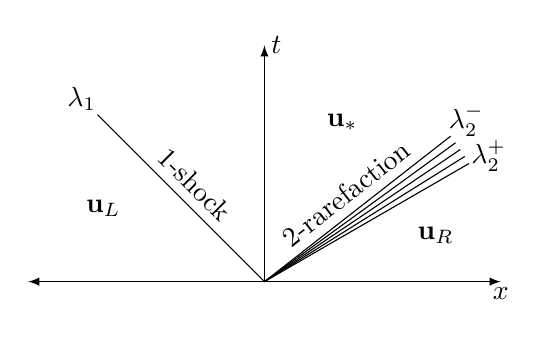
\begin{tikzpicture}[
  scale=1]

\def\mylength{3}

% axes
\draw[-latex] (0,0) -- (\mylength,0);
\draw[-latex] (0,0) -- (-\mylength,0);
\draw[-latex] (0,0) -- (0,\mylength);
\node at (0.15,\mylength) {$t$};
\node at (\mylength,-0.15) {$x$};

% characteristics
\draw (0,0) -- (30:\mylength);
\draw (0,0) -- (32:\mylength);
\draw (0,0) -- (34:\mylength);
\draw (0,0) -- (36:\mylength);
\draw (0,0) -- (38:\mylength) node[pos=0.5,sloped,above] {2-rarefaction};
\draw (0,0) -- (135:\mylength) node[pos=0.5,sloped,above] {1-shock};
\node at ($(135:\mylength)+(-0.2,0.2)$) {$\lambda_1$};
\node at ($(38:\mylength)+(0.2,0.2)$) {$\lambda_2^-$};
\node at ($(30:\mylength)+(0.25,0.1)$) {$\lambda_2^+$};

% solution values
\node at (155.5:0.75*\mylength) {$\mathbf{u}_L$};
\node at (15:0.75*\mylength) {$\mathbf{u}_R$};
\node at (64:0.75*\mylength) {$\mathbf{u}_*$};

\end{tikzpicture}

    \end{center}
  \item For a general conservation law system of size $m$,
    \begin{equation}
      \maxwavespeed(\vectorsolution_L,\vectorsolution_R)
        = \max\pr{|\lambda_1^-|,|\lambda_m^+|} \eqp
    \end{equation}
  \item Then for the example above
    $\maxwavespeed(\vectorsolution_L,\vectorsolution_R)$ is the maximum of
    the shock speed $|\lambda_1|$ and rarefaction \emph{head} speed $|\lambda_2^+|$.
\end{itemize}

\end{frame}
%%%%%%%%%%%%%%%%%%%%%%%%%%%%%%%%%%%%%%%%%%%%%%%%%%%%%%%%%%%%%%%%%%%%%%%%%%%%%%%%%
\begin{frame}
\frametitle{Maximum Wave Speeds (Cont.)}

\begin{itemize}
  \item For the SWE, a left \textcolor{secondarycolorheavy}{shock} has the wave speed
\begin{equation}\label{eq:left_shockspeed}
  \wavespeed_1^-(\vectorsolution_L, \vectorsolution_R)
    = \velocityx_L - \speedofsound_L\pr{1 + \pr{
    \frac{(\height_* - \height_L)(\height_* + 2\height_L)}{2\height_L^2}}}^{\frac{1}{2}}
    \eqc
\end{equation}
    where $\speedofsound=\sqrt{\gravity\height}$ is the ``speed of sound'' for the SWE.
  \item A left \textcolor{secondarycolorheavy}{rarefaction} has the head wave speed
\begin{equation}\label{eq:leftwavespeed_rarefaction}
  \wavespeed_1^-(\vectorsolution_L, \vectorsolution_R)
    = \velocityx_L - \speedofsound_L
    \eqc
\end{equation}
  \item Note the shock speed depends on the intermediate (star-state) solution
    for height $\height_*$, which may be computed with the following steps:
    \begin{itemize}
      \item Apply Rankine-Hugoniot condition to shock(s)
      \item Apply Riemann invariant condition to rarefaction(s)
      \item Combine resulting expressions and solve nonlinear equation for
        $\height_*$
    \end{itemize}
\end{itemize}

\end{frame}

%%%%%%%%%%%%%%%%%%%%%%%%%%%%%%%%%%%%%%%%%%%%%%%%%%%%%%%%%%%%%%%%%%%%%%%%%%%%%%%%%
\subsection{High-Order Scheme}
%%%%%%%%%%%%%%%%%%%%%%%%%%%%%%%%%%%%%%%%%%%%%%%%%%%%%%%%%%%%%%%%%%%%%%%%%%%%%%%%%
\begin{frame}
\frametitle{High-Order Scheme}

\begin{itemize}
  \item The high-order scheme adds a high-order diffusion term:
    \begin{equation}
      \sum_j\consistentmassentry
        \frac{\solutionvector_j^{H,n+1}-\solutionvector_j^n}{\dt}
        + \sum_j\gradiententry\cdot\consfluxinterpolant_j^n
        + \textcolor{secondarycolorheavy}{
          \sum_j\diffusionmatrixletter\ij^{H,n}\solutionvector_j^n}
        = \ssrhs_i^n \eqc
    \end{equation}
  \item The high-order diffusion matrix is proportional to an entropy diffusion matrix
    and uses the low-order diffusion matrix as an upper bound:
    \begin{equation}
      \diffusionmatrixletter^{H,n}\ij \equiv \min(
        \diffusionmatrixletter^{\entropy,n}\ij,\diffusionmatrixletter^{L,n}\ij) \eqc
    \end{equation}
    where the entropy diffusion matrix is proportional to an entropy residual and
    entropy jump:
    \begin{equation}
      \diffusionmatrixletter^{\entropy,n}\ij \equiv
        \frac{\entropyresidualcoef\entropyresidual\ij^n
          + \entropyjumpcoef\entropyjump\ij^n}{\entropynormalization\ij^n} \eqp
    \end{equation}
\end{itemize}

\end{frame}
%%%%%%%%%%%%%%%%%%%%%%%%%%%%%%%%%%%%%%%%%%%%%%%%%%%%%%%%%%%%%%%%%%%%%%%%%%%%%%%%%
\begin{frame}
\frametitle{Entropy for the Shallow Water Equations}

\begin{itemize}
  \item For the SWE, the entropy is chosen to be the sum of kinetic and
    potential energy terms:
    \begin{equation}
      \entropy(\vectorsolution,\bathymetry)
        = \half\frac{\heightmomentum\cdot\heightmomentum}{\height}
          + \half\gravity\height\pr{\height+\bathymetry}
      \eqp
    \end{equation}
  \item The entropy flux is
    \begin{equation}
      \mathbf{\consfluxletter}^\entropy(\vectorsolution,\bathymetry)
        = \gravity(\height + \bathymetry)\heightmomentum
        + \half\frac{\pr{\heightmomentum\cdot\heightmomentum}\heightmomentum} 
        {\height^2}
      \eqp
    \end{equation}
  \item The entropy residual is
    \begin{equation}
      \entropyresidual(\vectorsolution^\timeindex, \vectorsolution^{\timeindex-1})
        \equiv \frac{\entropy(\vectorsolution^\timeindex)
        - \entropy(\vectorsolution^{\timeindex-1})}{\timestepsize^{\timeindex-1}}
        + \divergence\mathbf{\consfluxletter}^\entropy(\vectorsolution^\timeindex,
          \bathymetry)
      \eqp
    \end{equation}
\end{itemize}

\end{frame}

%%%%%%%%%%%%%%%%%%%%%%%%%%%%%%%%%%%%%%%%%%%%%%%%%%%%%%%%%%%%%%%%%%%%%%%%%%%%%%%%%
\subsection{FCT Scheme}
%%%%%%%%%%%%%%%%%%%%%%%%%%%%%%%%%%%%%%%%%%%%%%%%%%%%%%%%%%%%%%%%%%%%%%%%%%%%%%%%%
\begin{frame}
\frametitle{FCT Antidiffusive Flux Definition}

\begin{itemize}
  \item The antidiffusive fluxes $\correctionfluxvector_i$ are defined such that
    \begin{equation}
      \lumpedmassentry
        \frac{\textcolor{secondarycolorheavy}{\solutionvector_i^{H}}
          -\solutionvector_i^n}{\dt}
        + \sum_j\gradiententry\cdot\consfluxinterpolant_j^n
        + \sum_j\diffusionmatrixletter\ij^{L,n}\solutionvector_j^n
        = \ssrhs_i^n + \textcolor{secondarycolorheavy}{\correctionfluxvector_i}
      \eqc
    \end{equation}
   \item Subtracting the high-order scheme equation from this gives the
      definition of $\correctionfluxvector$:
      \begin{equation}
        \correctionfluxvector_i \equiv
          \lumpedmassentry
            \frac{\solutionvector_i^{H}-\solutionvector_i^n}{\dt}
          -\sum_j\consistentmassentry
            \frac{\solutionvector_j^{H}-\solutionvector_j^n}{\dt}
          +\sum_j(\diffusionmatrixletter\ij^{L,n}-\diffusionmatrixletter\ij^{H,n})
            \solutionvector_j^n
      \end{equation}
   \item Decomposing $\correctionfluxvector$ into internodal fluxes
      $\correctionfluxmatrix\ij$ such that $\sum_j \correctionfluxmatrix\ij =
      \correctionfluxvector_i$,
      \begin{equation}
        \correctionfluxmatrix\ij = -M\ij^C\pr{
            \frac{\solutionvector_j^{H}-\solutionvector_j^n}{\dt}
            -\frac{\solutionvector_i^{H}-\solutionvector_i^n}{\dt}
          }
          + (D\ij^{L,n}-D\ij^{H,n})(\solutionvector_j^n-\solutionvector_i^n) \eqp
      \end{equation}
\end{itemize}

\end{frame}
%%%%%%%%%%%%%%%%%%%%%%%%%%%%%%%%%%%%%%%%%%%%%%%%%%%%%%%%%%%%%%%%%%%%%%%%%%%%%%%%%
\begin{frame}
\frametitle{FCT Limitation Process for Systems}

\begin{itemize}
  \item Bounds to impose on FCT solution are unclear for systems case:
    \begin{itemize}
      \item For scalar case, a DMP was used, but no DMP exists for systems.
      \item The invariant domain property is not useful here
        because while the property is known to hold, the domain itself is not
        actually known.
    \end{itemize}
  \item One may want to impose physical bounds on some non-conservative
    set of variables.
  \item Limitation of conservative variables may not satisfy these bounds.
  \item Consider the following sets of variables for the 1-D SWE:
    \begin{itemize}
      \item \textcolor{secondarycolorheavy}{Conservative}:
        $\vectorsolution \equiv [\height,\height\velocityx]\transpose$
      \item \textcolor{secondarycolorheavy}{Primitive}:
        $\check{\vectorsolution} \equiv [\height,\velocityx]\transpose$
      \item \textcolor{secondarycolorheavy}{Characteristic}:
        $\hat{\vectorsolution} \equiv [\velocityx-2\speedofsound,
          \velocityx+2\speedofsound]\transpose$,
          where $\speedofsound\equiv\sqrt{\gravity\height}$
    \end{itemize}
  \item Results from literature suggest that limitation on a non-conservative
    set of variables may produce superior results.
\end{itemize}

\end{frame}
%%%%%%%%%%%%%%%%%%%%%%%%%%%%%%%%%%%%%%%%%%%%%%%%%%%%%%%%%%%%%%%%%%%%%%%%%%%%%%%%%
\begin{frame}
\frametitle{Limitation on Non-Conservative Variables}

\begin{itemize}
  \item Consider some non-conservative set of variables
    $\hat{\vectorsolution} = \mathbf{T}^{-1}(\vectorsolution)\vectorsolution$.
    \begin{itemize}
      \item For \textcolor{secondarycolorheavy}{conservative} variables,
        $\mathbf{T}(\vectorsolution)=\mathbb{I}$.
      \item For \textcolor{secondarycolorheavy}{characteristic} variables,
        $\mathbf{T}(\vectorsolution)$ is the matrix with right eigenvectors
        of the Jacobian matrix $\partial\consfluxvector/\partial\vectorsolution$
        as its columns.
    \end{itemize}
  \item The FCT scheme for limitation of conservative variables is
    \begin{equation}
      \lumpedmassentry
        \frac{\solutionvector_i^{n+1}-\solutionvector_i^n}{\dt}
        + \sum_j\gradiententry\cdot\consfluxinterpolant_j^n
        + \sum_j\diffusionmatrixletter\ij^{L,n}\solutionvector_j^n
        = \ssrhs_i^n + \sum_j\limitermatrix\ij\odot\correctionfluxmatrix\ij \eqp
    \end{equation}
  \item Applying a local transformation $\mathbf{T}^{-1}(\solutionvector_i^n)$ gives
    \begin{equation}
      \lumpedmassentry
        \frac{\hat{\solutionvector}_i^{n+1}-\hat{\solutionvector}_i^n}{\dt}
        + \sum_j\gradiententry\cdot\hat{\consfluxinterpolant}_j^n
        + \sum_j\diffusionmatrixletter\ij^{L,n}\hat{\solutionvector}_j^n
        = \hat{\ssrhs}_i^n + \sum_j\limitermatrix\ij\odot\hat{\correctionfluxmatrix}\ij
        \eqc
    \end{equation}
    where accents denote transformed quantities, for example,
    \begin{equation}
      \hat{\solutionvector}_j^k
        = \mathbf{T}^{-1}(\solutionvector_i^n)\solutionvector_j^k
      \eqc \quad
      \hat{\correctionfluxmatrix}\ij
        = \mathbf{T}^{-1}(\solutionvector_i^n)\correctionfluxmatrix\ij
      \eqp
    \end{equation}
\end{itemize}

\end{frame}
%%%%%%%%%%%%%%%%%%%%%%%%%%%%%%%%%%%%%%%%%%%%%%%%%%%%%%%%%%%%%%%%%%%%%%%%%%%%%%%%%
\begin{frame}
\frametitle{Limiting Coefficients}

\begin{itemize}
  \item Choose $\limitermatrix\ij$ to satisfy some solution bounds
    $\hat{\solutionvector}_{i}^\pm$ and then define corresponding
    antidiffusive flux bounds $\hat{\mathbf{\limitedfluxbound}}_i^\pm$:
    \begin{equation}
      \hat{\mathbf{\limitedfluxbound}}^-_i \leq
        \sum\limits_j \limitermatrix\ij\odot\hat{\correctionfluxmatrix}\ij \leq
        \hat{\mathbf{\limitedfluxbound}}^+_i
      \quad\Rightarrow\quad
      \hat{\solutionvector}_i^- \leq
        \hat{\solutionvector}_i^{n+1} \leq
        \hat{\solutionvector}_i^+ \quad \forall i \eqp
    \end{equation}
  \item Performing some algebra gives the definition
    \begin{equation}
      \hat{\mathbf{\limitedfluxbound}}_i^\pm \equiv
        \lumpedmassentry\frac{\hat{\solutionvector}_i^\pm
          -\hat{\solutionvector}_i^n}{\dt}
        + \sum_j\gradiententry\cdot\hat{\consfluxinterpolant}_j^n
        + \sum_j\diffusionmatrixletter\ij^{L,n}\hat{\solutionvector}_j^n
        - \hat{\ssrhs}_i^n \eqp
    \end{equation}
  \item As in the scalar case, negative and positive antidiffusive flux
    sums are required in the limiting coefficient definitions:
    \begin{equation}
      \hat{\correctionfluxletter}_i^{\componentindex,-} \equiv
        \sum\limits_{j:\hat{\correctionfluxentry}\ij^\componentindex<0}
        \hat{\correctionfluxentry}\ij^\componentindex \eqc \qquad
      \hat{\correctionfluxletter}_i^{\componentindex,+} \equiv
        \sum\limits_{j:\hat{\correctionfluxentry}\ij^\componentindex>0}
        \hat{\correctionfluxentry}\ij^\componentindex \eqp
    \end{equation}
\end{itemize}

\end{frame}
%%%%%%%%%%%%%%%%%%%%%%%%%%%%%%%%%%%%%%%%%%%%%%%%%%%%%%%%%%%%%%%%%%%%%%%%%%%%%%%%%
\begin{frame}
\frametitle{Limiting Coefficients (Cont.)}

\begin{itemize}
  \item The limiting coefficients are first computed just as in the scalar case:
    \begin{equation}
      \limiterletter_i^{\componentindex,\pm} \equiv\left\{
        \begin{array}{l l}
          1 & \hat{\correctionfluxletter}_i^{\componentindex,\pm} = 0\\
          \min\left(1,\frac{Q_i^{\componentindex,\pm}}
            {\hat{\correctionfluxletter}_i^{\componentindex,\pm}}\right) &
          \hat{\correctionfluxletter}_i^{\componentindex,\pm} \ne 0
        \end{array}
      \right. \eqp
    \end{equation}
    \begin{equation}
      \limiterletter\ij^\componentindex \equiv\left\{
        \begin{array}{l l}
          \min(L_i^{\componentindex,+},L_j^{\componentindex,-}) &
            \hat{\correctionfluxentry}\ij^\componentindex \geq 0\\
          \min(L_i^{\componentindex,-},L_j^{\componentindex,+}) &
            \hat{\correctionfluxentry}\ij^\componentindex < 0
        \end{array}
      \right. \eqp
    \end{equation}
  \item However, there is a caveat: limiting coefficients may require
    \hlorange{synchronization}, e.g.,
    \begin{equation}
      \limiterletter\ij^\componentindex \mapsfrom
        \min\limits_k\limiterletter\ij^k \quad \forall\componentindex \eqp
    \end{equation}
  \item Otherwise, antidiffusive fluxes in one component can violate the
    conditions of another component.
\end{itemize}

\end{frame}

%%%%%%%%%%%%%%%%%%%%%%%%%%%%%%%%%%%%%%%%%%%%%%%%%%%%%%%%%%%%%%%%%%%%%%%%%%%%%%%%%
\section{Shallow Water Equations Results}
%%%%%%%%%%%%%%%%%%%%%%%%%%%%%%%%%%%%%%%%%%%%%%%%%%%%%%%%%%%%%%%%%%%%%%%%%%%%%%%%%
\begin{frame}
\frametitle{1-D Dam Break Test Problem}
\framesubtitle{Height, 256 cells, FE}

\begin{center}
\includegraphics[height=0.8\textheight]{./figures/dambreak1d_Height_FE_256cells.pdf}
\end{center}

\end{frame}
%%%%%%%%%%%%%%%%%%%%%%%%%%%%%%%%%%%%%%%%%%%%%%%%%%%%%%%%%%%%%%%%%%%%%%%%%%%%%%%%%
\begin{frame}
\frametitle{1-D Dam Break Test Problem}
\framesubtitle{Discharge, 256 cells, FE}

\begin{center}
\includegraphics[height=0.8\textheight]{./figures/dambreak1d_Momentum_FE_256cells.pdf}
\end{center}

\end{frame}
%%%%%%%%%%%%%%%%%%%%%%%%%%%%%%%%%%%%%%%%%%%%%%%%%%%%%%%%%%%%%%%%%%%%%%%%%%%%%%%%%
\begin{frame}
\frametitle{1-D Dam Break Test Problem}
\framesubtitle{Height, 256 cells, SSPRK33}

\begin{center}
\includegraphics[height=0.8\textheight]{./figures/dambreak1d_Height_SSP3_256cells.pdf}
\end{center}

\end{frame}
%%%%%%%%%%%%%%%%%%%%%%%%%%%%%%%%%%%%%%%%%%%%%%%%%%%%%%%%%%%%%%%%%%%%%%%%%%%%%%%%%
\begin{frame}
\frametitle{1-D Dam Break Test Problem}
\framesubtitle{Discharge, 256 cells, SSPRK33}

\begin{center}
\includegraphics[height=0.8\textheight]{./figures/dambreak1d_Momentum_SSP3_256cells.pdf}
\end{center}

\end{frame}
%%%%%%%%%%%%%%%%%%%%%%%%%%%%%%%%%%%%%%%%%%%%%%%%%%%%%%%%%%%%%%%%%%%%%%%%%%%%%%%%%
\begin{frame}
\frametitle{Bathtub Test Problem}
\framesubtitle{Height, 4096 cells, FE}

\begin{figure}[h]
   \centering
   \begin{subfigure}{0.3\textwidth}
      \centering
      \includegraphics[width=0.8\textwidth]{./figures/bathtub_initial_shape.png}
      \caption{Initial Shape}
   \end{subfigure}
   \begin{subfigure}{0.3\textwidth}
      \centering
      \includegraphics[width=0.8\textwidth]{./figures/bathtub_low_t01.png}
      \caption{Low-order, $t=0.1$}
   \end{subfigure}
   \begin{subfigure}{0.3\textwidth}
      \centering
      \includegraphics[width=0.8\textwidth]{./figures/bathtub_low_t05.png}
      \caption{Low-order, $t=0.5$}
   \end{subfigure}
   \begin{subfigure}{0.3\textwidth}
      \centering
      \includegraphics[width=0.8\textwidth]{./figures/bathtub_initial.png}
      \caption{$t=0$}
   \end{subfigure}
   \begin{subfigure}{0.3\textwidth}
      \centering
      \includegraphics[width=0.8\textwidth]{./figures/bathtub_EV_t01.png}
      \caption{EV, $t=0.1$}
   \end{subfigure}
   \begin{subfigure}{0.3\textwidth}
      \centering
      \includegraphics[width=0.8\textwidth]{./figures/bathtub_EV_t05.png}
      \caption{EV, $t=0.5$}
   \end{subfigure}
\end{figure}

\end{frame}
%%%%%%%%%%%%%%%%%%%%%%%%%%%%%%%%%%%%%%%%%%%%%%%%%%%%%%%%%%%%%%%%%%%%%%%%%%%%%%%%%
\begin{frame}
\frametitle{2-D Dam Break Test Problem}
\framesubtitle{Initial Height}

\begin{center}
\includegraphics[height=0.8\textheight]{./figures/dambreak2d_initial.png}
\end{center}

\end{frame}
%%%%%%%%%%%%%%%%%%%%%%%%%%%%%%%%%%%%%%%%%%%%%%%%%%%%%%%%%%%%%%%%%%%%%%%%%%%%%%%%%
\begin{frame}
\frametitle{2-D Dam Break Test Problem}
\framesubtitle{Height, $t=50$, SSPRK33}

\begin{figure}[h]
   \centering
   \begin{subfigure}{0.49\textwidth}
      \centering
      \includegraphics[width=\textwidth]{./figures/dambreak2d_height_Low.png}
      \caption{Low-order}
   \end{subfigure}
   \begin{subfigure}{0.49\textwidth}
      \centering
      \includegraphics[width=\textwidth]{./figures/dambreak2d_height_EV.png}
      \caption{EV}
   \end{subfigure}
\end{figure}

\end{frame}
%%%%%%%%%%%%%%%%%%%%%%%%%%%%%%%%%%%%%%%%%%%%%%%%%%%%%%%%%%%%%%%%%%%%%%%%%%%%%%%%%
\begin{frame}
\frametitle{2-D Dam Break Test Problem}
\framesubtitle{Height Surface, Colored by Discharge, $t=50$, SSPRK33}

\begin{figure}[h]
   \centering
   \begin{subfigure}{0.49\textwidth}
      \centering
      \includegraphics[width=\textwidth]{./figures/dambreak2d_height_Low_surface.png}
      \caption{Low-order}
   \end{subfigure}
   \begin{subfigure}{0.49\textwidth}
      \centering
      \includegraphics[width=\textwidth]{./figures/dambreak2d_height_EV_surface.png}
      \caption{EV}
   \end{subfigure}
\end{figure}

\end{frame}
%%%%%%%%%%%%%%%%%%%%%%%%%%%%%%%%%%%%%%%%%%%%%%%%%%%%%%%%%%%%%%%%%%%%%%%%%%%%%%%%%
\begin{frame}
\frametitle{2-D Dam Break Test Problem}
\framesubtitle{Viscosity Profiles, $t=50$, SSPRK33}

\begin{figure}[h]
   \centering
   \begin{subfigure}{0.49\textwidth}
      \centering
      \includegraphics[width=\textwidth]{./figures/dambreak2d_low_order_viscosity_logscale.png}
      \caption{Low-order}
   \end{subfigure}
   \begin{subfigure}{0.49\textwidth}
      \centering
      \includegraphics[width=\textwidth]{./figures/dambreak2d_entropy_viscosity_logscale.png}
      \caption{EV}
   \end{subfigure}
\end{figure}

\end{frame}


In conclusion, the FCT scheme presented guarantees
a non-negative solution that satisfies a discrete maximum principle.
While this FCT scheme does not guarantee monotonicity, it has been
found to be successful in many simple test problems. The underlying
high-order scheme based on entropy viscosity has been found to
produce a higher quality FCT solution than using an inviscid
high-order scheme. A number of challenges remain - for example,
FCT transients can give rise to spurious plateaus and can have non-monotone
solutions within the bounds of the imposed discrete maximum principle.
These unphysical effects arise due to unphysical oscillations in the
high-order solution; improving the high-order solution improves
the quality of the FCT scheme.

Future work will extend this scheme to implicit time
discretizations since the CFL condition required by explicit time
discretizations can be very restrictive, particularly for radiation transport simulations.
In addition, many problems of interest involve steady-state solutions
of the transport equation, so a steady-state FCT scheme will also be
a subject of future work.


%%%%%%%%%%%%%%%%%%%%%%%%%%%%%%%%%%%%%%%%%%%%%%%%%%%%%%%%%%%%%%%%%%%%%%%%%%%%%%%%
\begin{frame}
\frametitle{Acknowledgments}

\begin{itemize}
   \item Dr. Jean Ragusa
   \item Dr. Jean-Luc Guermond
   \item Dr. Bojan Popov
   \item Dr. Marco Delchini
   \item Dr. Richard Martineau
\end{itemize}
\begin{itemize}
   \item This material is based upon work supported under an Integrated University
      Program Graduate Fellowship.
\end{itemize}

\begin{center}
   \includegraphics[width=0.4\textwidth]{./figures/NEUP_Final_Logo_Version-09.jpg}
\end{center}
\end{frame}

%%%%%%%%%%%%%%%%%%%%%%%%%%%%%%%%%%%%%%%%%%%%%%%%%%%%%%%%%%%%%%%%%%%%%%%%%%%%%%%%%
\section{Backup Slides}
%%%%%%%%%%%%%%%%%%%%%%%%%%%%%%%%%%%%%%%%%%%%%%%%%%%%%%%%%%%%%%%%%%%%%%%%%%%%%%%%%
\begin{frame}
\frametitle{Strong-Stability-Preserving Runge-Kutta Methods}

\begin{itemize}
  \item A general $s$-stage SSPRK method for discretizing a system
    $\massmatrix\ddt{\solutionvector} = \ssres(\solutionvector,t)$
    is the following:
    \begin{equation}
      \solutionvector^{n+1} = \RKstagesolution^{s} \eqc
    \end{equation}
    \begin{equation}
      \RKstagesolution^i = \left\{\begin{array}{l l}
        \solutionvector^n & i = 0\\
        \RKoldsolutioncoef_i\RKstagesolution^0
        + \RKstagesolutioncoef_i\RKintermediatesolution^i & i\ne 0
      \end{array}\right. \eqc 
    \end{equation}
    \begin{equation}
      \massmatrix\RKintermediatesolution^i = \massmatrix\RKstagesolution^{i-1}
        + \timestepsize\,\ssres(\RKstagetime_i,\RKstagesolution^{i-1})
      \eqc
    \end{equation}
    where $\RKstagetime_i = \timevalue^\timeindex+\RKtimecoef_i\timestepsize$,
  \item An example is the Shu-Osher method (3-stage, 3rd-order-accurate):
    \begin{equation}
      \RKoldsolutioncoef = \left[\begin{array}{c}
        0\\\frac{3}{4}\\\frac{1}{3}\end{array}\right]
        \qquad\RKstagesolutioncoef = \left[\begin{array}{c}
        1\\\frac{1}{4}\\\frac{2}{3}\end{array}\right]
        \qquad c = \left[\begin{array}{c}0\\1\\\frac{1}{2}\end{array}\right] \eqp
    \end{equation}
\end{itemize}

\end{frame}
%%%%%%%%%%%%%%%%%%%%%%%%%%%%%%%%%%%%%%%%%%%%%%%%%%%%%%%%%%%%%%%%%%%%%%%%%%%%%%%%%
\begin{frame}
\frametitle{Low-Order Steady-State Matrix Row Sum}

\begin{itemize}
  \item Recall that $\ssmatrixletter\ij^{L,n}\equiv\ssmatrixletter\ij^{n}
    +\diffusionmatrixletter\ij^{L,n}$. Thus,
      $\sumj\ssmatrixletter\ij^{L,n} = \sumj\ssmatrixletter\ij^{n}
      +\sumj\diffusionmatrixletter\ij^{L,n} \eqp$
  \item Recall the zero-row-sum property of $\diffusionmatrix^{L,n}$:
    \begin{equation}
      \diffusionmatrixletter_{i,i}^{L,n} =
        -\sum_{j\ne i}\diffusionmatrixletter_{i,j}^{L,n}
      \eqc \quad \Rightarrow \quad
        \sumj\diffusionmatrixletter_{i,j}^{L,n} = 0 \eqp
    \end{equation}
  \item Thus $\sumj\ssmatrixletter^{L,n}\ij =
   \sumj \ssmatrixletter^{\timeindex}\ij$:
\begin{equation}
  \sumj\ssmatrixletter^{L,n}\ij = \sumj \intSi
    \left(\mathbf{\consfluxletter}'(\approximatescalarsolution^\timeindex)
      \cdot\nabla\testfunction_j(\x) +
      \reactioncoef(\x)\testfunction_j(\x)\right)\testfunction_i(\x) d\volume \eqp
\end{equation}
  \item Now, using the fact that $\sumj\testfunction_j(\x)=1$
    (and $\nabla 1 = 0$) gives
    \begin{equation}
      \sumj\ssmatrixletter^{L,n}\ij =
        \intSi\reactioncoef(\x)\testfunction_i(\x) d\volume \eqp
    \end{equation}
\end{itemize}

\end{frame}
%%%%%%%%%%%%%%%%%%%%%%%%%%%%%%%%%%%%%%%%%%%%%%%%%%%%%%%%%%%%%%%%%%%%%%%%%%%%%%%%%
\begin{frame}
\frametitle{Limiting Coefficients Definition}

\begin{itemize}
   \item The classic Zalesak limiting strategy starts by separating the
      negative and positive fluxes:
      \begin{equation}
         Q^-_i \leq \sum\limits_{j:\correctionfluxij<0} L\ij \correctionfluxij +
            \sum\limits_{j:\correctionfluxij>0} L\ij \correctionfluxij\leq Q^+_i \eqp
      \end{equation}
   \item Zalesak's limiting coefficients assume that
      all positive fluxes into a node $i$ have the same limiting coefficient
      $L^+_i$ and similarly, negative fluxes have the same limiting coefficient
      $L^-_i$:
      \begin{equation}
        Q^-_i \leq L^-_i \correctionfluxletter^-_i
          + L^+_i \correctionfluxletter^+_i \leq Q^+_i \eqp
      \end{equation}
      where
      \begin{equation}
        \correctionfluxletter_i^- \equiv \sum\limits_{j:\correctionfluxij<0}
          \correctionfluxij \eqc \qquad
        \correctionfluxletter_i^+ \equiv \sum\limits_{j:\correctionfluxij>0}
          \correctionfluxij \eqp
      \end{equation}
   \item As a conservative bound for $L^+_i$, contributions from negative fluxes
      are ignored (pretending $L_i^-=0$), giving
      $L^+_i \leq \frac{Q_i^+}{\correctionfluxletter_i^+}$
      and similarly for $L^-_i$ and the lower bound.
\end{itemize}

\end{frame}
%%%%%%%%%%%%%%%%%%%%%%%%%%%%%%%%%%%%%%%%%%%%%%%%%%%%%%%%%%%%%%%%%%%%%%%%%%%%%%%%%
\begin{frame}
\frametitle{Limiting Coefficients Definition (Cont.)}

\begin{itemize}
   \item Then, recalling that limiting coefficients are not greater than unity:
      \begin{equation}
         L_i^\pm \equiv\left\{
            \begin{array}{l l}
               1 & \correctionfluxletter_i^\pm = 0\\
               \min\left(1,\frac{Q_i^\pm}{\correctionfluxletter_i^\pm}\right) &
                 \correctionfluxletter_i^\pm \ne 0
            \end{array}
            \right. \eqp
      \end{equation}
   \item However, to limit fluxes conservatively, limited correction fluxes must
      be equal and opposite:
      \begin{equation}
        L\ij \correctionfluxij = -L_{j,i}
          \MakeUppercase{\correctionfluxletter}_{j,i} \eqp
      \end{equation}
      Since $\correctionfluxij$ happens to be skew symmetric
      ($\MakeUppercase{\correctionfluxletter}_{j,i}=-\correctionfluxij$) due to the
      chosen flux decomposition, the limiting coefficients must be symmetric:
      $L_{j,i} = L\ij$.
\end{itemize}

\end{frame}
%%%%%%%%%%%%%%%%%%%%%%%%%%%%%%%%%%%%%%%%%%%%%%%%%%%%%%%%%%%%%%%%%%%%%%%%%%%%%%%%%
\begin{frame}
\frametitle{Limiting Coefficients Definition (Cont.)}

\begin{itemize}
   \item Thus when deciding the limiting coefficient $L\ij$ for a flux $\correctionfluxij$, 
      one must not only consider the bounds for $i$ but also the bounds for $j$.
      Specifically, a positive flux $\correctionfluxij$ risks violating $Q_i^+$ and $Q_j^-$.
      Putting everything together,
      \begin{equation}
         L\ij \equiv\left\{
            \begin{array}{l l}
               \min(L_i^+,L_j^-) & \correctionfluxij \geq 0\\
               \min(L_i^-,L_j^+) & \correctionfluxij < 0
            \end{array}
            \right. \eqp
      \end{equation}
\end{itemize}

\end{frame}
%%%%%%%%%%%%%%%%%%%%%%%%%%%%%%%%%%%%%%%%%%%%%%%%%%%%%%%%%%%%%%%%%%%%%%%%%%%%%%%%%%
%\begin{frame}
%\frametitle{Comparison of Time Discretizations}
%\framesubtitle{CFL = 0.8, 32 cells}
%
%\begin{center}
%   \includegraphics[width=0.8\textwidth]
%     {\contentdir/results/transport/time_methods/compare_time_methods.pdf}
%\end{center}
%
%\end{frame}
%%%%%%%%%%%%%%%%%%%%%%%%%%%%%%%%%%%%%%%%%%%%%%%%%%%%%%%%%%%%%%%%%%%%%%%%%%%%%%%%%%
%\begin{frame}
%\frametitle{Backward Euler Galerkin FCT for Different CFL Numbers}
%
%\begin{center}
%   \includegraphics[width=0.9\textwidth]
%     {\contentdir/results/transport/compare_cfl/compare_cfl.pdf}
%\end{center}
%
%\end{frame}
%%%%%%%%%%%%%%%%%%%%%%%%%%%%%%%%%%%%%%%%%%%%%%%%%%%%%%%%%%%%%%%%%%%%%%%%%%%%%%%%%
\begin{frame}
\frametitle{Discrete Maximum Principle Bounds for a Theta-Scheme}

\begin{itemize}
\item Recall the DMP bounds 
  $\DMPlowerbound_i\leq \solutionletter_i^{L,\timeindex+1}\leq \DMPupperbound_i$
  for explicit Euler:
      \begin{equation}
         W_i^\pm \equiv U_{\substack{\max\\\min},i}^n\left(
         1-\frac{\dt}{M_{i,i}^L}
         \sum\limits_j A\ij^{L,n}\right)
         + \frac{\Delta t}{M_{i,i}^L}b_i^n \eqp
      \end{equation}
\item In contrast, the DMP bounds for the $\theta$ scheme are implicit:
\begin{subequations}
\begin{multline}\label{eq:theta_bounds}
   \DMPbounds_i
   \equiv \frac{1}{1+\frac{\theta\timestepsize}{\massmatrixletter^L_{i,i}}
     \ssmatrixletter_{i,i}^{L,\timeindex+1}}\Bigg[\pr{1
     - \frac{(1-\theta)\timestepsize}{\massmatrixletter^L_{i,i}}
       \sumj\ssmatrixletter_{i,j}^{L,\timeindex}}
       \solutionletter_{\substack{\max\\\min},i}^\timeindex\\
     - \frac{\theta\timestepsize}{\massmatrixletter^L_{i,i}}
       \sumjnoti\ssmatrixletter_{i,j}^{L,\timeindex+1}
       \solutionletter_{\substack{\max\\\min},i}^{L,\timeindex+1}
     + \frac{\timestepsize}{\massmatrixletter^L_{i,i}}\pr{(1-\theta)
       \ssrhsletter_i^\timeindex + \theta\ssrhsletter_i^{\timeindex+1}}\Bigg] \eqc
\end{multline}
\begin{equation}
  \solutionletter_{\substack{\max\\\min},i}^\timeindex
  = \substack{\max\\\min\limits_{j\in\indices(\support_i)}}
    \solutionletter_j^\timeindex
  \eqc \quad
  \solutionletter_{\substack{\max\\\min},i}^{L,\timeindex+1}
  = \substack{\max\\\min\limits_{j\in\indices(\support_i)}}
  \solutionletter_j^{L,\timeindex+1}
  \eqp
\end{equation}
\end{subequations}
\end{itemize}

\end{frame}
%%%%%%%%%%%%%%%%%%%%%%%%%%%%%%%%%%%%%%%%%%%%%%%%%%%%%%%%%%%%%%%%%%%%%%%%%%%%%%%%%
\begin{frame}
\frametitle{1-D Dam Break Test Problem}
\framesubtitle{Phase Diagram, FE, 32 cells}

\begin{center}
   \includegraphics[width=0.9\textwidth]
     {figures/phase_all_FE_32cells.pdf}
\end{center}

\end{frame}

%%%%%%%%%%%%%%%%%%%%%%%%%%%%%%%%%%%%%%%%%%%%%%%%%%%%%%%%%%%%%%%%%%%%%%%%%%%%%%%%%
\end{document}
